\documentclass{beamer}
\usepackage{multimedia}
\usepackage{hyperref}
\usetheme{Madrid}
\usepackage{multicol}
\usepackage{caption}
\usepackage{makecell}
\usepackage{xcolor, colortbl, soul}
\sethlcolor{yellow}

\makeatother
\setbeamertemplate{footline}
{
  \leavevmode%
  \hbox{%
  \begin{beamercolorbox}[wd=.17\paperwidth,ht=2.25ex,dp=1ex,center]{author in head/foot}%
    \usebeamerfont{author in head/foot}\insertshortauthor
  \end{beamercolorbox}%
  \begin{beamercolorbox}[wd=.59\paperwidth,ht=2.25ex,dp=1ex,center]{title in head/foot}%
    \usebeamerfont{title in head/foot}\insertshorttitle\hspace*{3em}
  \end{beamercolorbox}}%
  \begin{beamercolorbox}[wd=.24\paperwidth,ht=2.25ex,dp=1ex,right]{date in head/foot}%
    \usebeamerfont{date in head/foot}\insertshortdate{}\hspace*{2em}
    \insertframenumber{} / \inserttotalframenumber\hspace*{2ex} 
  \end{beamercolorbox}%

  \vskip0pt%
}
\makeatletter
\setbeamertemplate{navigation symbols}{}


\title[Multiple Manipulations on Clothes Images with MANN]{\large Multiple Manipulations on Clothes Images with MAN}
\author[Francesco Fantechi]{Francesco Fantechi \\ \vspace{0.2cm} \scriptsize Relatore: Alberto Del Bimbo \\ Corelatore: Federico Becattini}
\date[UNIFI 2022-2023]{\footnotesize A.A. 2022-2023}

\institute[]{

\begin{figure}[!h]
\centering
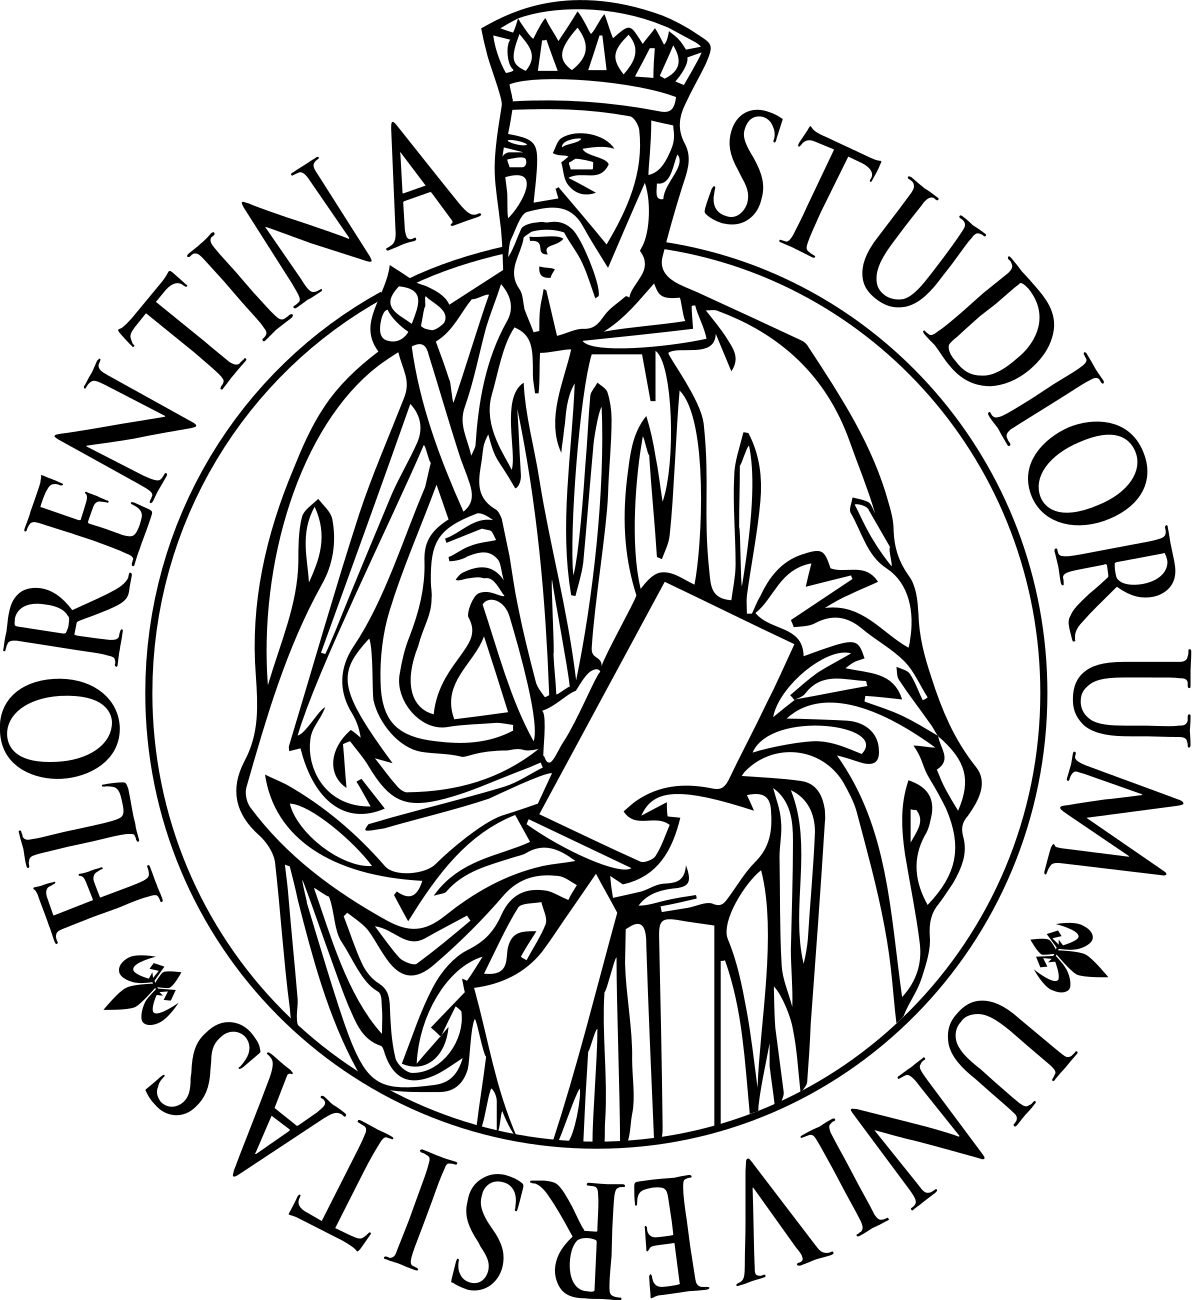
\includegraphics[width=1.9cm, height=1.9cm]{"Immagini/LogoUnifi.PNG"}
\end{figure}

%\begin{center}
UNIVERSITA' DEGLI STUDI DI FIRENZE \\
Facolta di Ingegneria \\
Corso di Laurea Magistrale in Ingegneria Informatica
%\end{center}
}

\begin{document}

\frame{\titlepage}

\begin{frame}
\frametitle{Introduzione}
\begin{columns}
\column{0.4\textwidth}
\begin{itemize} 
\item <1-> Compiere manipolazioni su immagini di vestiti per un negozio online di moda
\begin{itemize} 
	\item <2-> Esempio: rimuovere il colletto, la chiusura e allungare le maniche dal vestito di sinistra
\end{itemize} 
\item <3-> Un'interazione pu\'o impattare in modo eccessivo anche altri aspetti dell'immagine stravolgendola pi\'u del dovuto

\end{itemize}
\column{0.6\textwidth}
\begin{itemize}
	\item[] <1|only@1> 
		\begin{figure}[!h]
 			\begin{center}
 			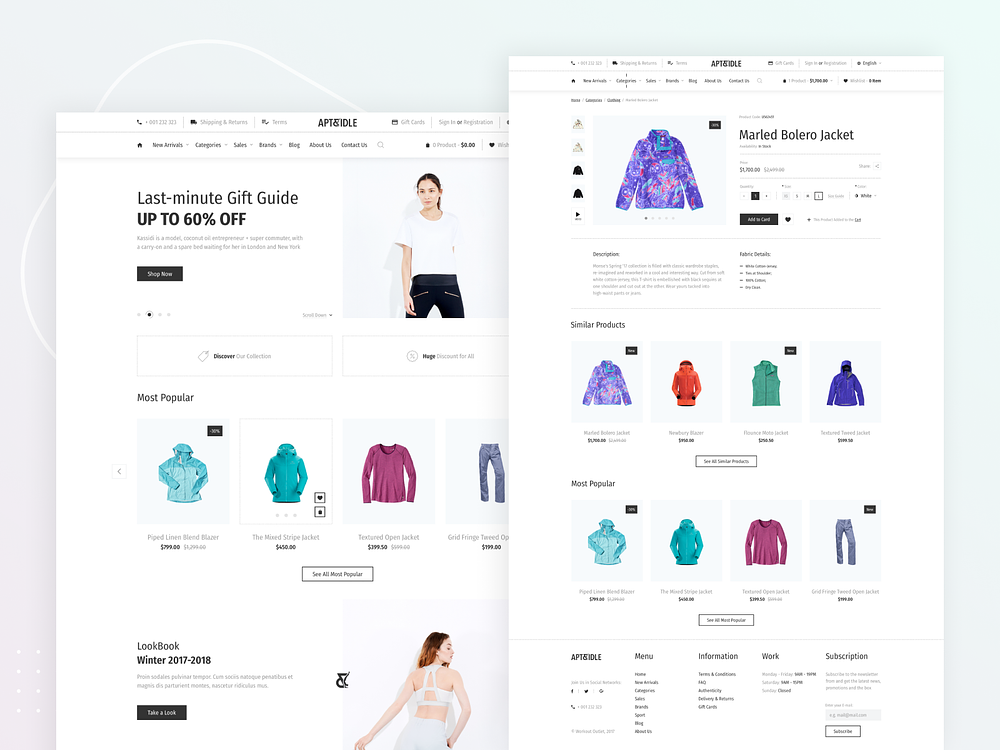
\includegraphics[scale=0.18]{"Immagini/Store.png"}
 			\end{center}
 		\end{figure}
 	\item[] <2|only@2> 
		\begin{figure}[!h]
 			\begin{center}
 			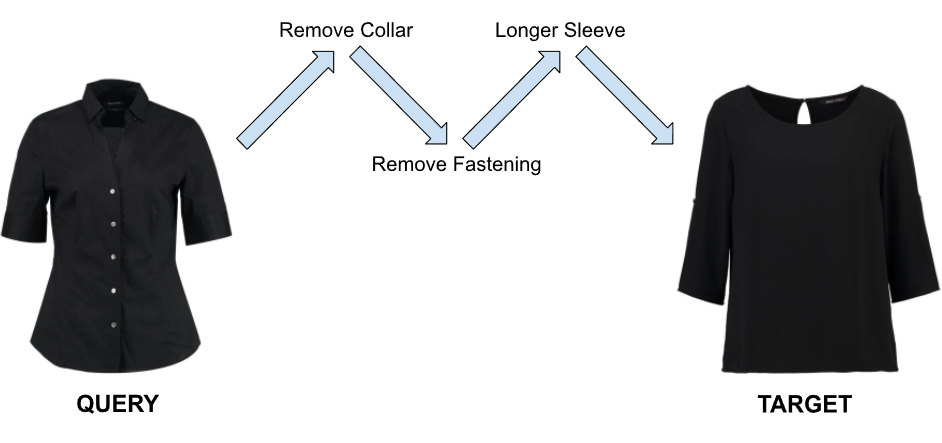
\includegraphics[scale=0.19]{"Immagini/Sample.png"}
 			\end{center}
 		\end{figure}
 	\item[] <3|only@3> 
		\begin{figure}[!h]
 			\begin{center}
 			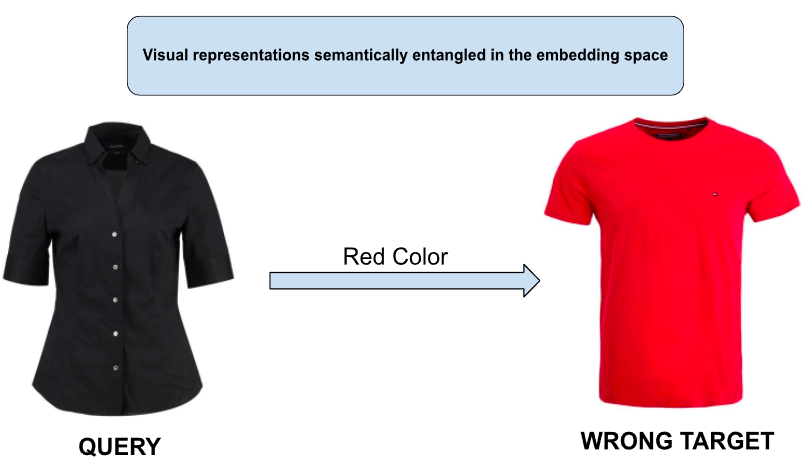
\includegraphics[scale=0.22]{"Immagini/Wrong.png"}
 			\end{center}
 		\end{figure}
\end{itemize}
\end{columns}
\end{frame}

\begin{frame}
\frametitle{Soluzione proposta da Amazon}
\begin{columns}
\column{0.35\textwidth}
\begin{itemize} 
\item <1-> Attribute-Driven Disentangled Encoder (ADDE) per ottenere una rappresentazione visuale meno correlata nello sapzio degli attributi
\item <2-> ADDE-M, ADDE $+$ Memory Block
\item <3-> Supporta una sola manipolazione alla volta

\end{itemize}
\column{0.65\textwidth}
\begin{itemize}
	\item[] <1|only@1> 
		\begin{figure}[!h]
 			\begin{center}
 			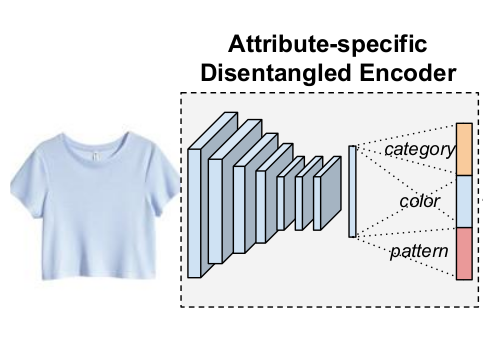
\includegraphics[scale=0.35]{"Immagini/ASDE.png"}
 			\end{center}
 		\end{figure}
 	\item[] <2|only@2> 
		\begin{figure}[!h]
 			\begin{center}
 			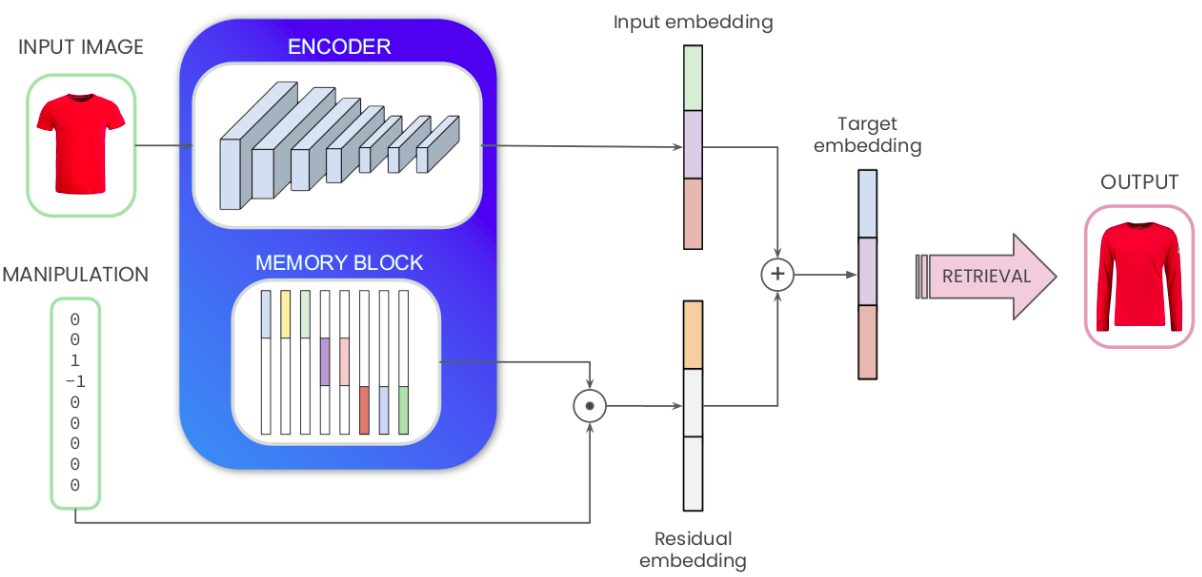
\includegraphics[scale=0.17]{"Immagini/ADDE-M_Simplified.png"}
 			\end{center}
 		\end{figure}
 	\item[] <3|only@3> 
		\begin{figure}[!h]
 			\begin{center}
 			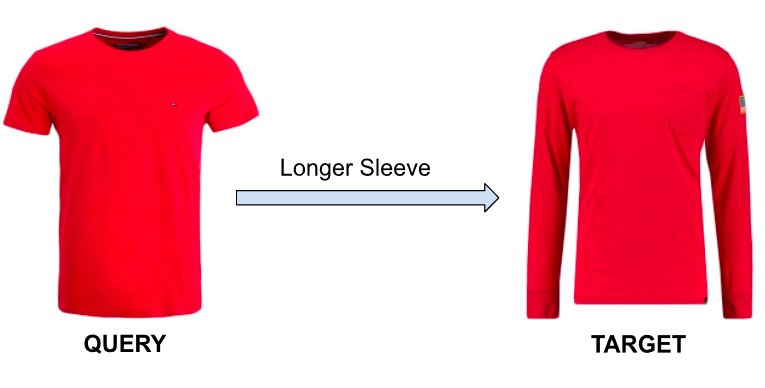
\includegraphics[scale=0.22]{"Immagini/One_Manipulation.png"}
 			\end{center}
 		\end{figure}
\end{itemize}
\end{columns}
\end{frame}

\begin{frame}
\frametitle{La nostra proposta}
\begin{columns}
\column{0.35\textwidth}
\begin{itemize} 
\item <1-> Memory Augmented Neural Network (MANN)
\begin{itemize} 
	\item <2-> Memoria esterna indipendente con il ruolo di base di conoscenza
	\item <3-> Controller che impara ad interagire con essa leggendo e scrivendo per produrre l'output
\end{itemize}
\end{itemize}
\column{0.65\textwidth}

		\begin{figure}[!h]
 			\begin{center}
 			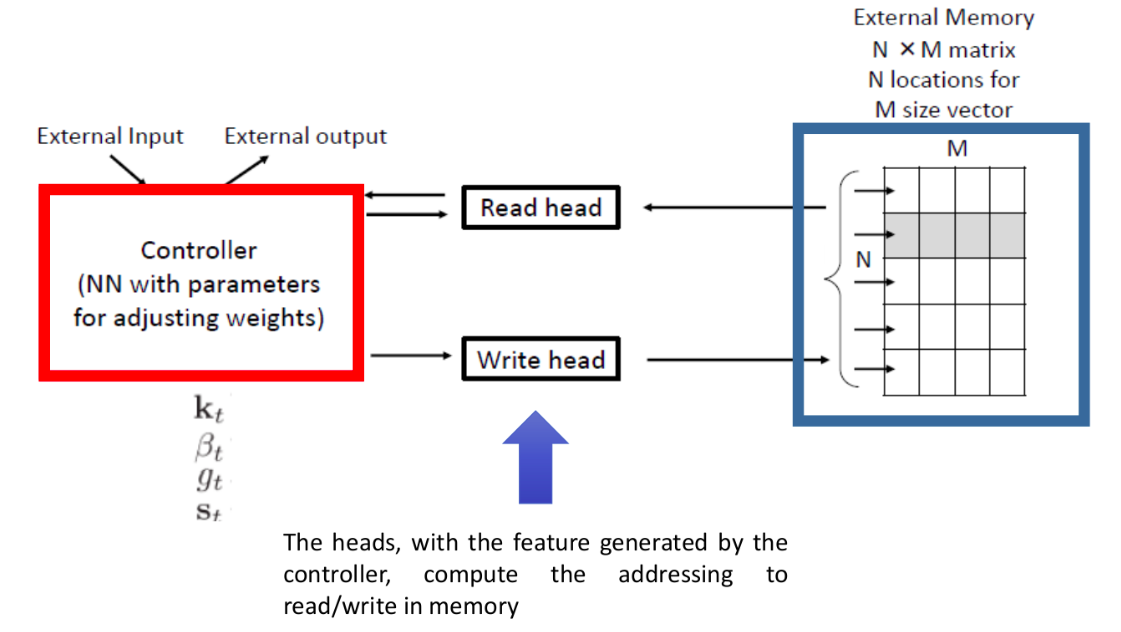
\includegraphics[scale=0.18]{"Immagini/MANN.png"}
 			\end{center}
 		\end{figure}
\end{columns}
\end{frame}

\begin{frame}
\frametitle{La nostra proposta}
\begin{columns}
\column{0.5\textwidth}
\begin{itemize} 
\item <1-> Neural Turing Machine (NTM)
\item <2-> Modello IGOR
\item <3-> Content Based Addressing
\item <4-> Read:\\ \footnotesize	 $r_{t}=\sum_{i=0}^{N-1}\omega_{t}(i)M_{t}(i)$
\item <5-> Write:\\ \scriptsize $M_{t}(i)=M_{t-1}(i)(1-\omega_{t}(i)e_{t})+\omega_{t}(i)a_{t}$

\end{itemize}
\column{0.5\textwidth}
\begin{itemize}
	\item[] <1|only@1> 
		\begin{figure}[!h]
 			\begin{center}
 			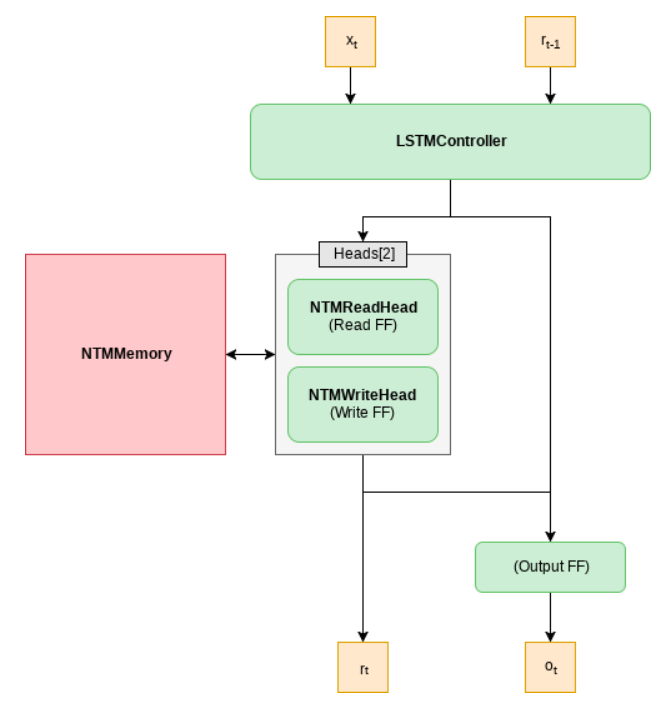
\includegraphics[scale=0.22]{"Immagini/NTM.png"}
 			\end{center}
 		\end{figure}
 	\item[] <2|only@2> 
		\begin{figure}[!h]
 			\begin{center}
 			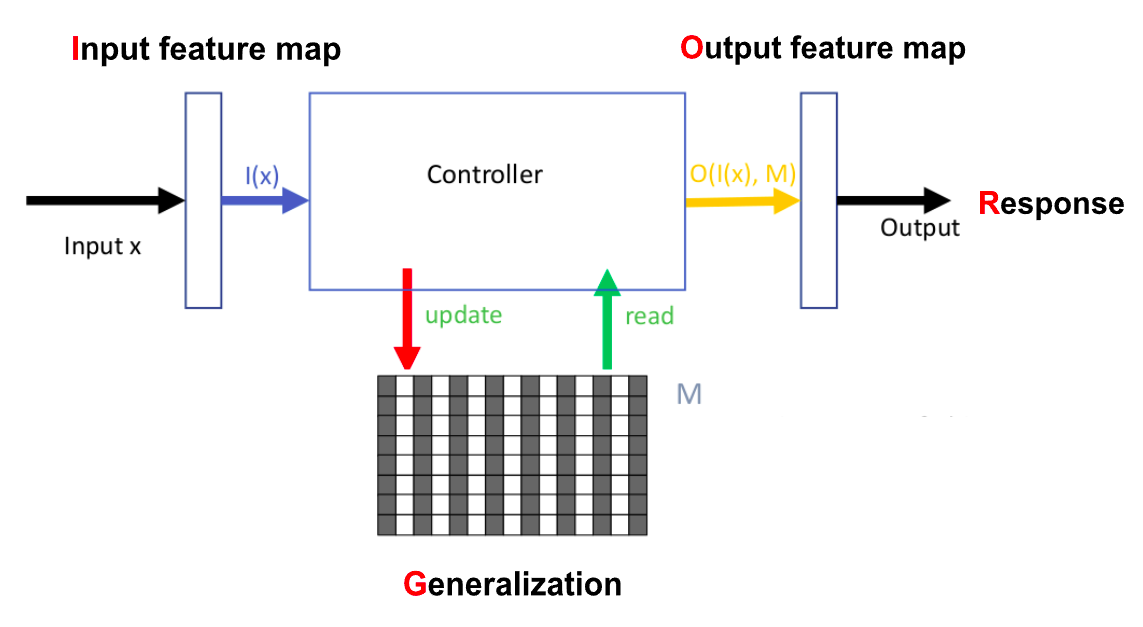
\includegraphics[scale=0.135]{"Immagini/IGOR.png"}
 			\end{center}
 		\end{figure}
 	\item[] <3|only@3> 
		\begin{figure}[!h]
 			\begin{center}
 			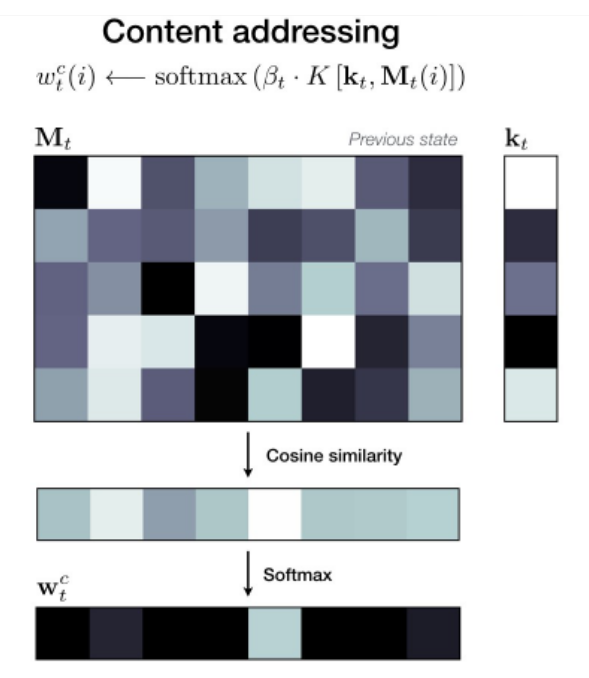
\includegraphics[scale=0.22]{"Immagini/CBA.png"}
 			\end{center}
 		\end{figure}
 	\item[] <4|only@4> 
		\begin{figure}[!h]
 			\begin{center}
 			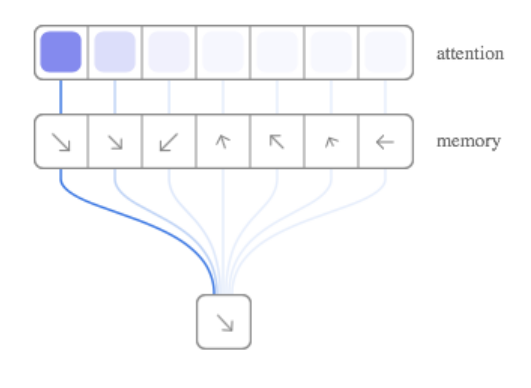
\includegraphics[scale=0.24]{"Immagini/Read.png"}
 			\end{center}
 		\end{figure}
 	\item[] <5|only@5> 
		\begin{figure}[!h]
 			\begin{center}
 			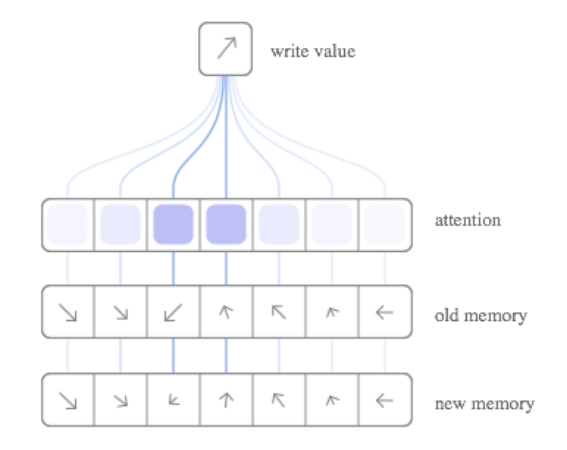
\includegraphics[scale=0.24]{"Immagini/Write.png"}
 			\end{center}
 		\end{figure}
\end{itemize}
\end{columns}
\end{frame}

\begin{frame}
\frametitle{Vantaggi}
\begin{itemize} 
\item <1-> Grande memoria indipendente e indirizzabile
\begin{itemize}
	\item <2-> Supporta $N >= 1$ manipolazioni in sequenza
	\item <3-> Maggior supervisione sul comportamento interno della rete 
	\item <4-> Modello semplice e numero di parametri contenuto
\end{itemize}
\item[] <1|only@1> 
\begin{figure}[!h]
 			\begin{center}
 			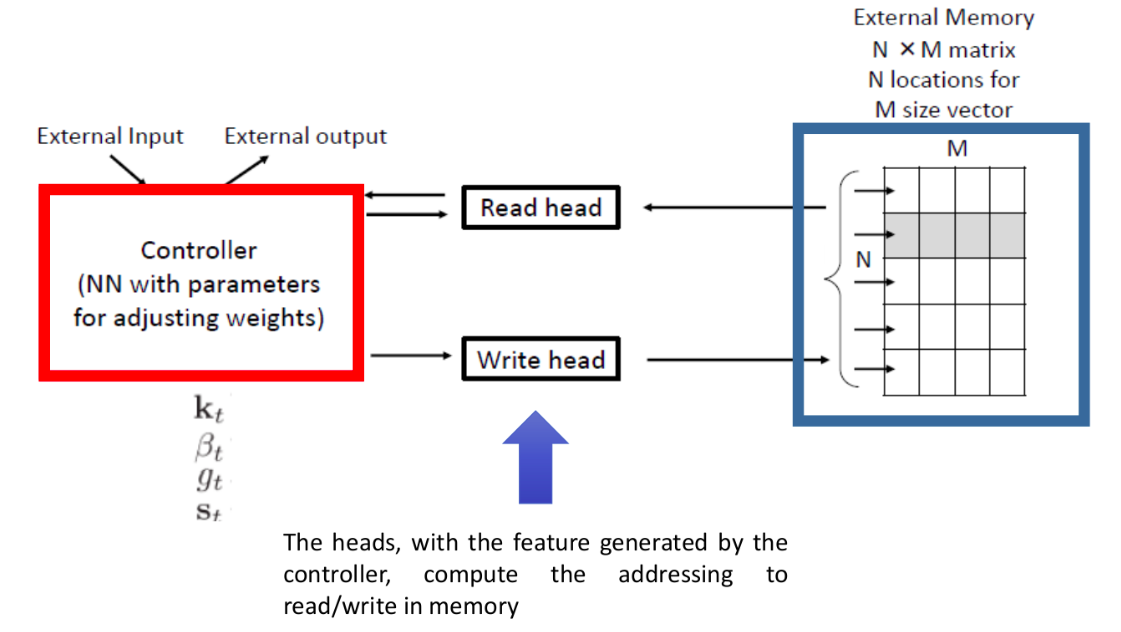
\includegraphics[scale=0.18]{"Immagini/MANN.png"}
 			\end{center}
\end{figure}
\item[] <2|only@2> 
\begin{figure}[!h]
 			\begin{center}
 			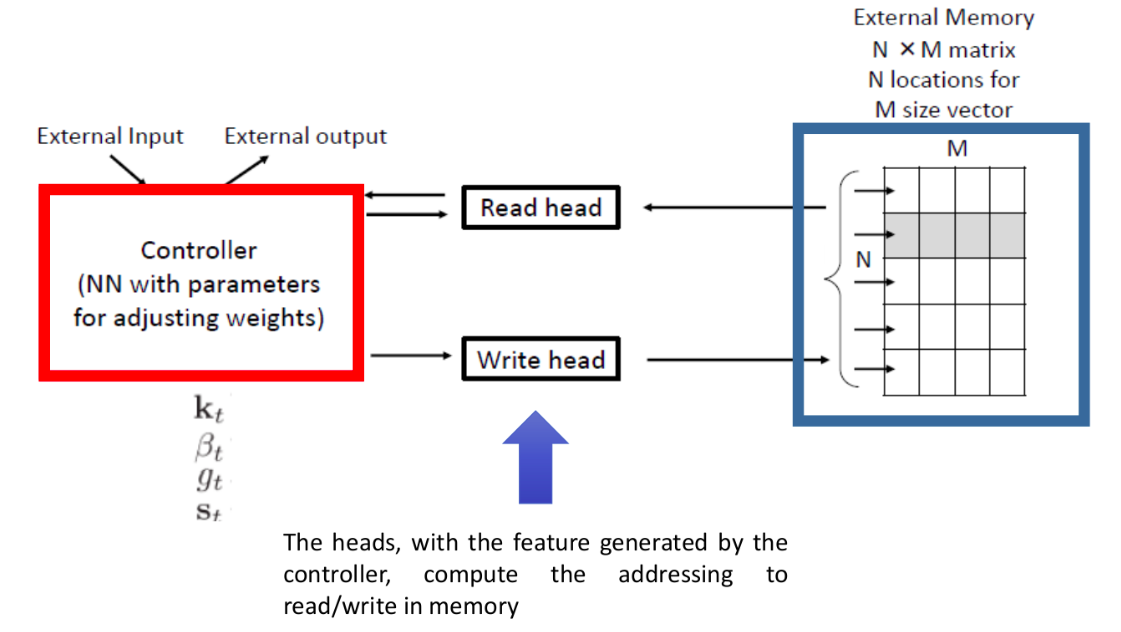
\includegraphics[scale=0.18]{"Immagini/MANN.png"}
 			\end{center}
\end{figure}
\item[] <3|only@3> 
\begin{figure}[!h]
 			\begin{center}
 			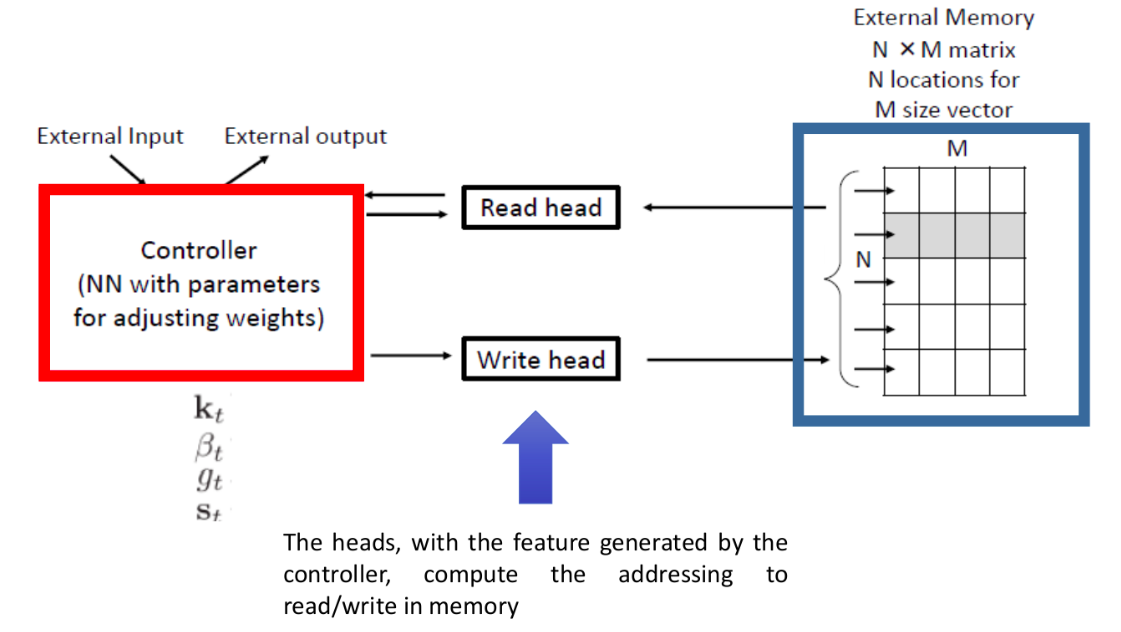
\includegraphics[scale=0.18]{"Immagini/MANN.png"}
 			\end{center}
\end{figure}
\item[] <4|only@4> 
\begin{figure}[!h]
 			\begin{center}
 			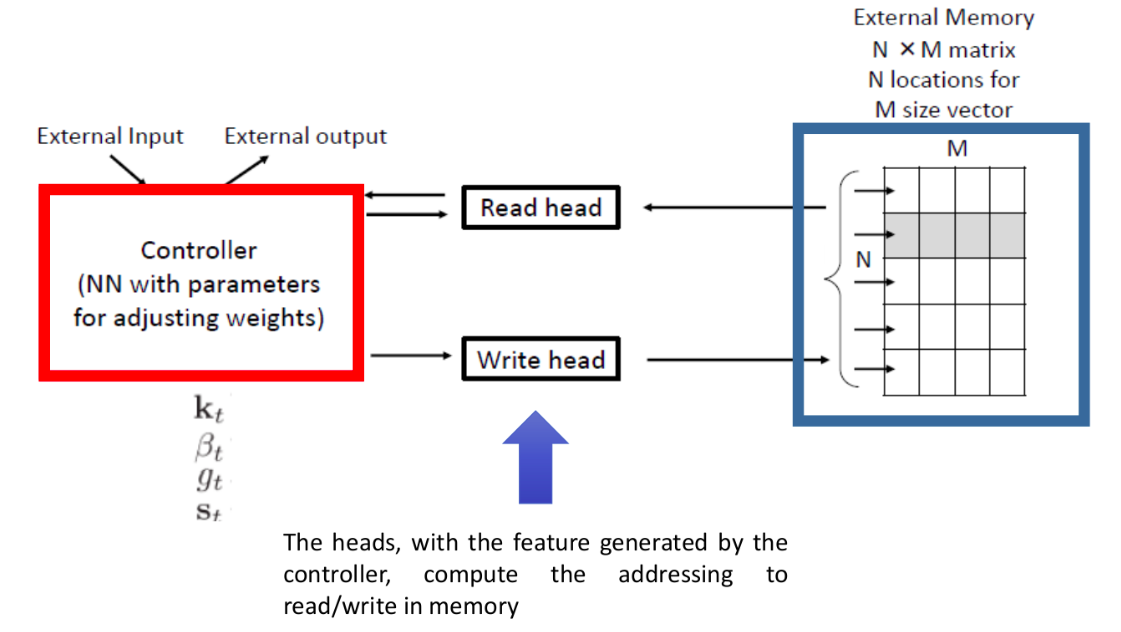
\includegraphics[scale=0.18]{"Immagini/MANN.png"}
 			\end{center}
\end{figure}
\end{itemize}
\end{frame}

\begin{frame}
\frametitle{Addestramento}
\begin{itemize} 
\item <1-> Dataset Shopping100k
\begin{itemize}
	\item <2-> $80586$ immagini di addestramento
	\item <3-> $20000$ immagini di test
	\item <4-> Ogni immagine è caratterizzata attraverso $12$ attributi a ognuno dei quali \'e associato un certo numero di etichette
\end{itemize}
\item <5-> La rete \'e stata addestrata su migliaia di esempi
\item <6-> Ogni esempio (immagine query e target a distanza $<= 8$) \'e stato generato randomicamente real time di modo da ridurre la possibilit\'a di overfitting
\item <7-> Ad ogni nuovo esempio la memoria esterna viene inizializzata con il vettore "disentangled" dell'immagine query
\item <8-> Dopo aver avuto in input $N <= 8$ manipolazioni la memoria contiene il vettore da confrontare con quello dell'immagine target
\item <9-> Utilizzo della libreria Tensorboard per monitorare l'andamento dell'addestramento
\end{itemize}
\end{frame}

\begin{frame}
\frametitle{Addestramento}
\begin{figure}[!h]
 			\begin{center}
 			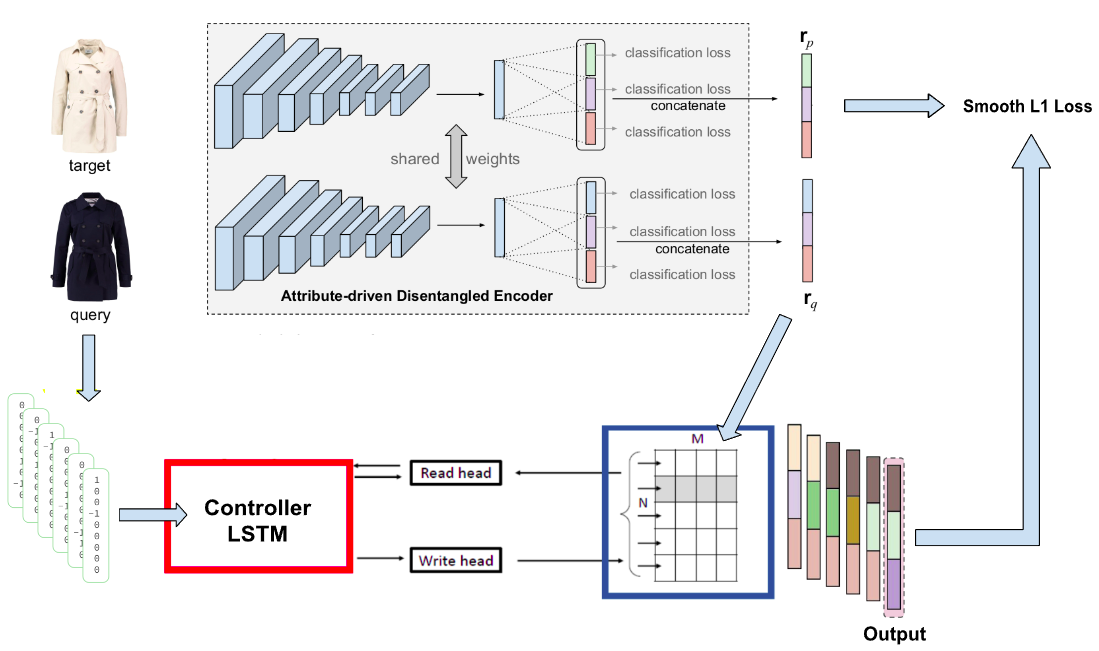
\includegraphics[scale=0.3]{"Immagini/All2.png"}
 			\end{center}
\end{figure}
\end{frame}

\begin{frame}
\frametitle{Risultati}
\begin{itemize} 
\item <1-> Test di Amazon: $\thickapprox 1400$ coppie a distanza $=1$
\item[] <1|only@1> 
\captionof{table}{Top-k retrieval accuracies on Shopping100k for attribute manipulation}
\hspace{15px}
\begin{tabular}{|c|c|c|c|c|c|}
\hline
\multicolumn{6}{|c|}{Shopping100k}\\
\hline
\thead{} & \thead{Top-10} & \thead{Top-20} & \thead{Top-30} & \thead{Top-40} & \thead{Top-50}\\
\hline
\thead{AMNet} & \thead{$ 25.62 $}  & \thead{$ 36.13 $} & \thead{$ 42.94 $} & \thead{$ 47.71 $} & \thead{$ 51.64 $}\\
\hline
\thead{ADDE-M} & \thead{$ 41.17 $}  & \thead{$ 52.93 $} & \thead{$ 59.81 $} & \thead{$ 64.10 $} & \thead{$ 67.29 $}\\
\hline
\thead{MANN} & \thead{$ 33.58 $}  & \thead{$ 44.96 $} & \thead{$ 52.00 $} & \thead{$ 56.72 $} & \thead{$ 60.18 $}\\
\hline
\end{tabular}
\end{itemize}
\end{frame}

\begin{frame}
\frametitle{Risultati}
\begin{itemize} 
\item Confronto visuale MANN e ADDE-M con $1$ manipolazione
\item[] <1|only@1> 
\hspace{-20px}
\begin{figure}[!h]
 			\begin{center}
 			\hspace{-70px}
 			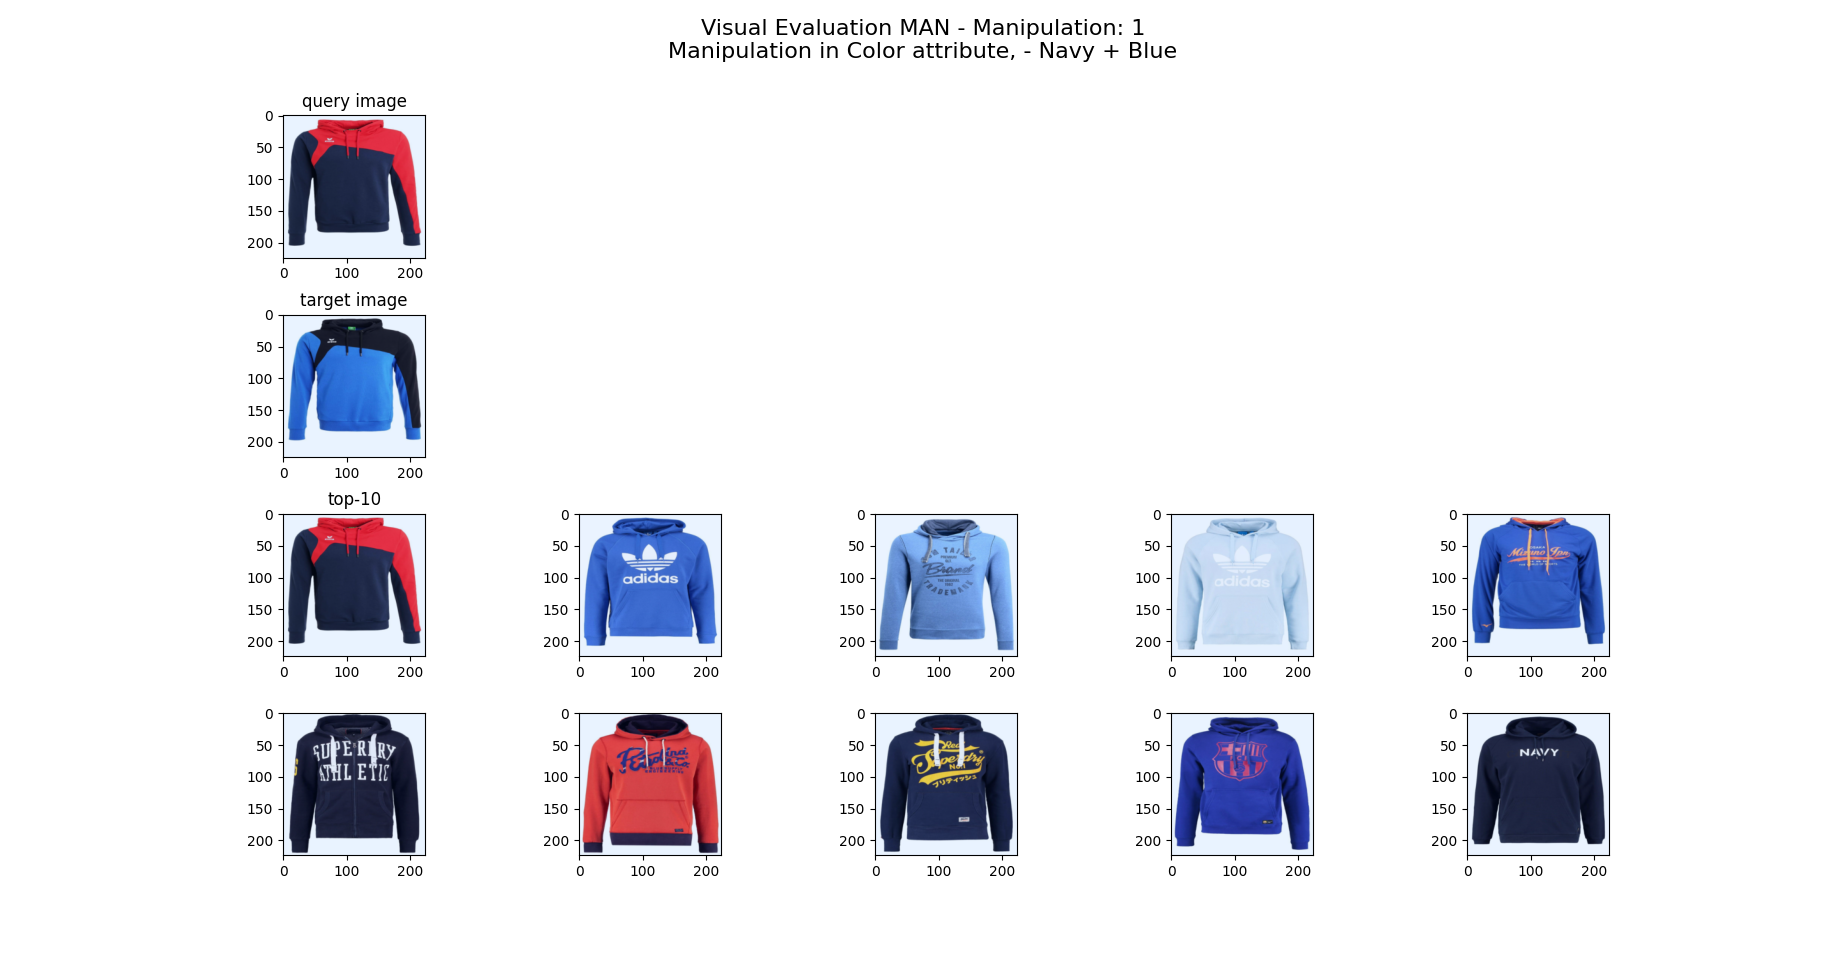
\includegraphics[scale=0.29]{"Immagini/1_MANN.png"}
 			\end{center}
\end{figure}
\item[] <2|only@2>
\hspace{-20px} 
\begin{figure}[!h]
 			\begin{center}
 			\hspace{-70px}
 			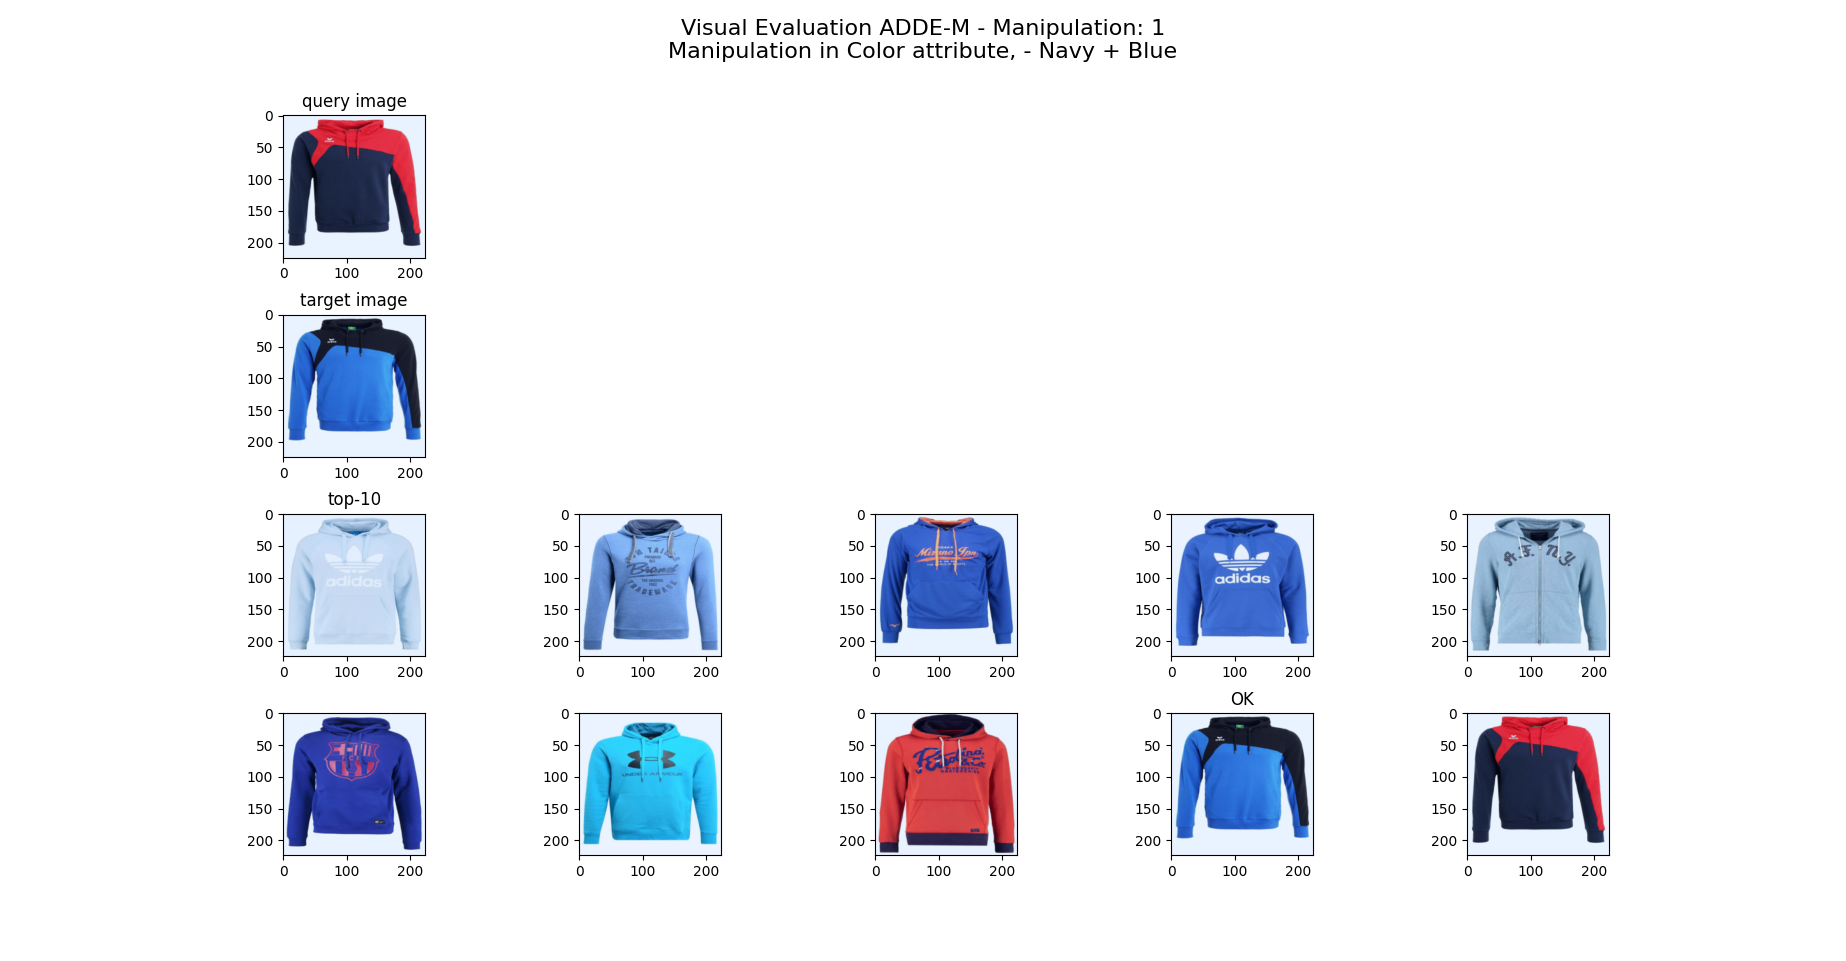
\includegraphics[scale=0.29]{"Immagini/1_ADDEM.png"}
 			\end{center}
\end{figure}
\end{itemize}
\end{frame}

\begin{frame}
\frametitle{Risultati}
\begin{itemize} 
\item <1-> Test di Amazon: $\thickapprox 1400$ coppie a distanza $=1$
\captionof{table}{Normalized Discounted Cumulative Gain metrics}
\hspace{90px}
\begin{tabular}{|c|c|c|c|c|c|}
\hline
\multicolumn{3}{|c|}{Shopping100k}\\
\hline
\thead{} & \thead{ADDE-M} & \thead{MANN} \\
\hline
\thead{$NDCG@30$} & \thead{$ 0.7367 $} & \thead{$ 0.7448 $}\\
\hline
\thead{$NDCG_{t}@30$} & \thead{$ 0.4305 $} & \thead{$ 0.3259 $}\\
\hline
\thead{$NDCG_{o}@30$} & \thead{$ 0.7779 $} & \thead{$ 0.7987 $}\\
\hline
\end{tabular}
\item <1-> $NDCG=\frac{1}{Z}\sum_{j=1}^{k}\frac{2^{rel(j)-1}}{log(j+1)}$
\item <1-> $rel(j)$ \'e il punteggio di rilevanza sugli attributi della i-esima immagine \footnotesize (numero di attributi che matchano con il ground-truth diviso per il numero totale di attributi)
\item <1-> $NDCG_{t}@30$, $rel(j)$ calcolato solo su attributi manipolati
\item <1-> $NDCG_{o}@30$, $rel(j)$ calcolato solo su attributi non manipolati
\end{itemize}
\end{frame}

\begin{frame}
\frametitle{Risultati}
\begin{itemize} 
\item $1$ Loss: Smooth L1 Loss
\end{itemize}
\begin{figure}[!h]
 			\begin{center}
 			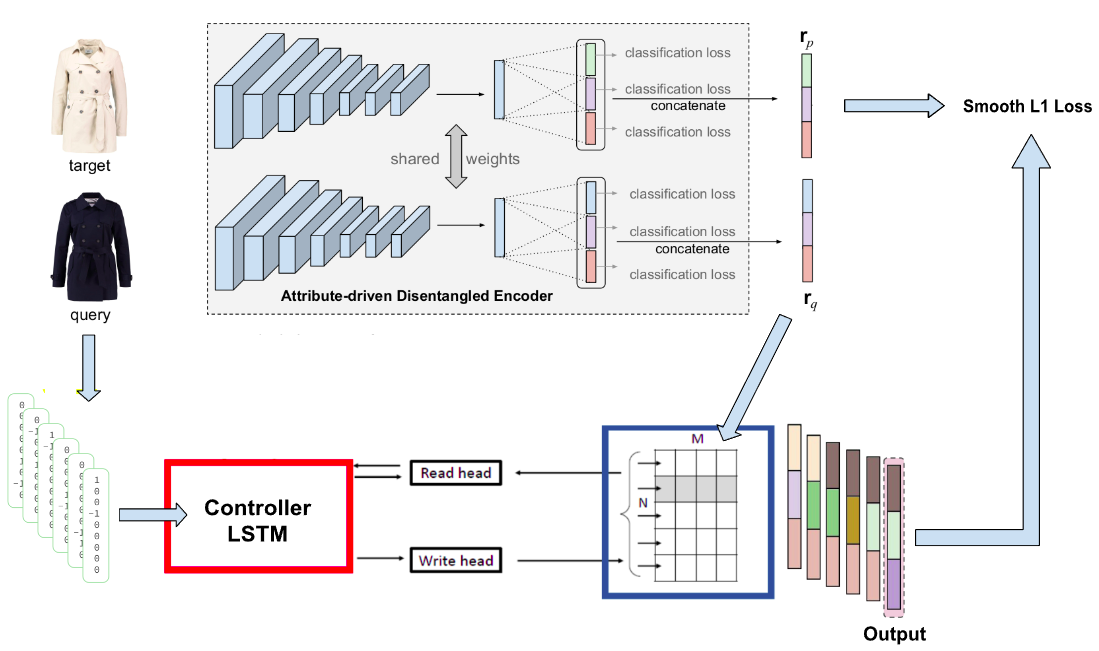
\includegraphics[scale=0.3]{"Immagini/All2.png"}
 			\end{center}
\end{figure}
\end{frame}

\begin{frame}
\frametitle{Risultati}
\begin{itemize} 
\item $3$ Loss: Triplet Loss, Consistency Loss e Label Triplet Loss
\end{itemize}
\begin{figure}[!h]
 			\begin{center}
 			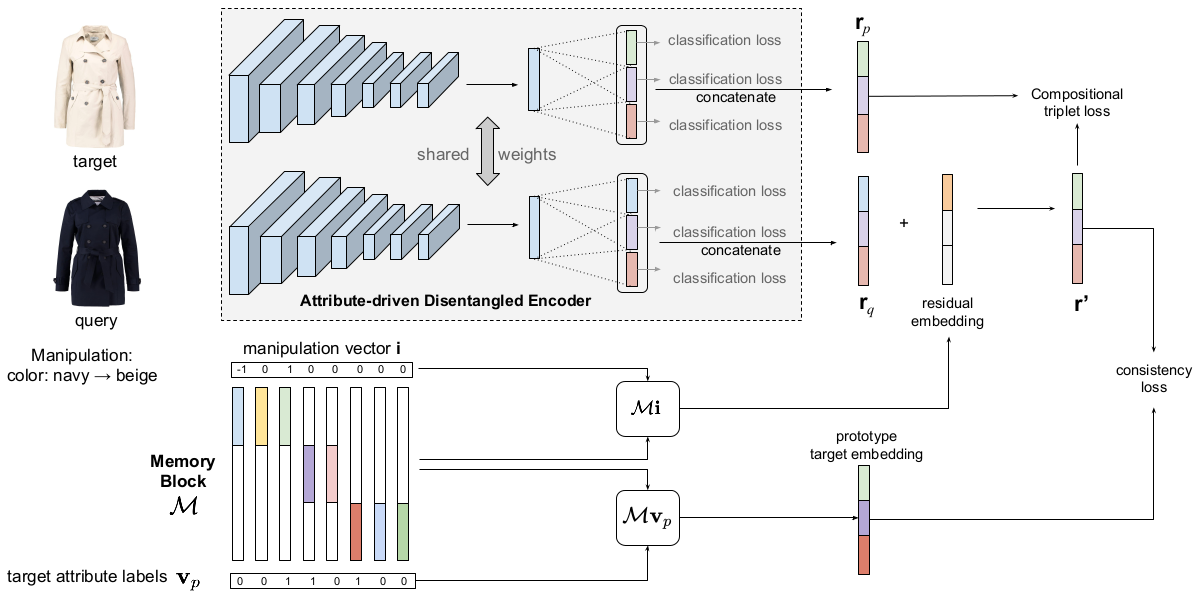
\includegraphics[scale=0.29]{"Immagini/ADDE-M.png"}
 			\end{center}
\end{figure}
\end{frame}

\begin{frame}
\frametitle{Risultati}
\begin{itemize} 
\item <1-> Il nostro test: $1000$ coppie a distanza $\leq 8$
\item[] <1|only@1> 
\captionof{table}{Top-k retrieval accuracies on Shopping100k for attribute manipulation}
\hspace{15px}
\begin{tabular}{|c|c|c|c|c|c|}
\hline
\multicolumn{6}{|c|}{Shopping100k}\\
\hline
\thead{} & \thead{Top-10} & \thead{Top-20} & \thead{Top-30} & \thead{Top-40} & \thead{Top-50}\\
\hline
\thead{ADDE-M} & \thead{$ 2.0 $}  & \thead{$ 4.0 $} & \thead{$ 5.0 $} & \thead{$ 6.0 $} & \thead{$ 7.0 $}\\
\hline
\thead{MANN} & \thead{$ 33.0 $}  & \thead{$ 45.0 $} & \thead{$ 52.00 $} & \thead{$ 56.0 $} & \thead{$ 60.0 $}\\
\hline
\end{tabular}
\end{itemize}
\end{frame}

\begin{frame}
\frametitle{Risultati}
\begin{itemize} 
\item Confronto visuale MANN e ADDE-M con $3$ manipolazioni
\item[] <1|only@1> 
\hspace{-20px}
\begin{figure}[!h]
 			\begin{center}
 			\hspace{-80px}
 			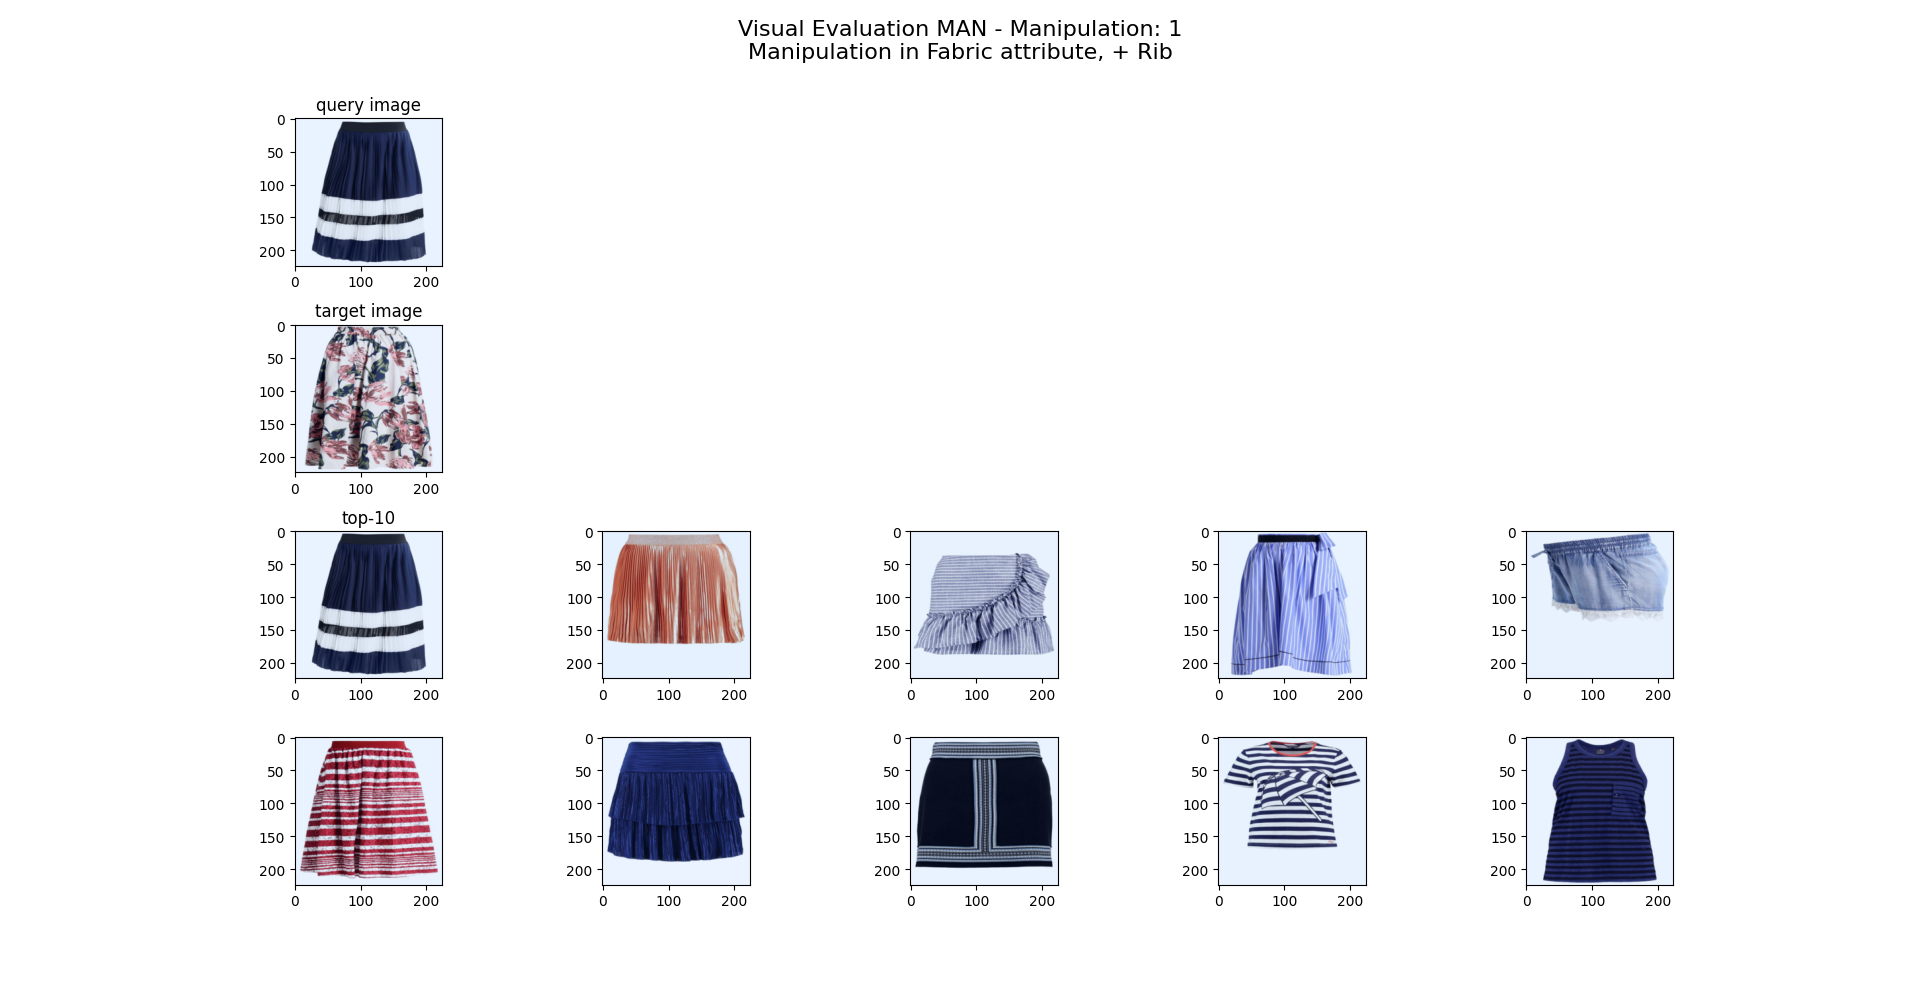
\includegraphics[scale=0.28]{"Immagini/3.1.png"}
 			\end{center}
\end{figure}
\item[] <2|only@2>
\hspace{-20px}
\begin{figure}[!h]
 			\begin{center}
 			\hspace{-80px}
 			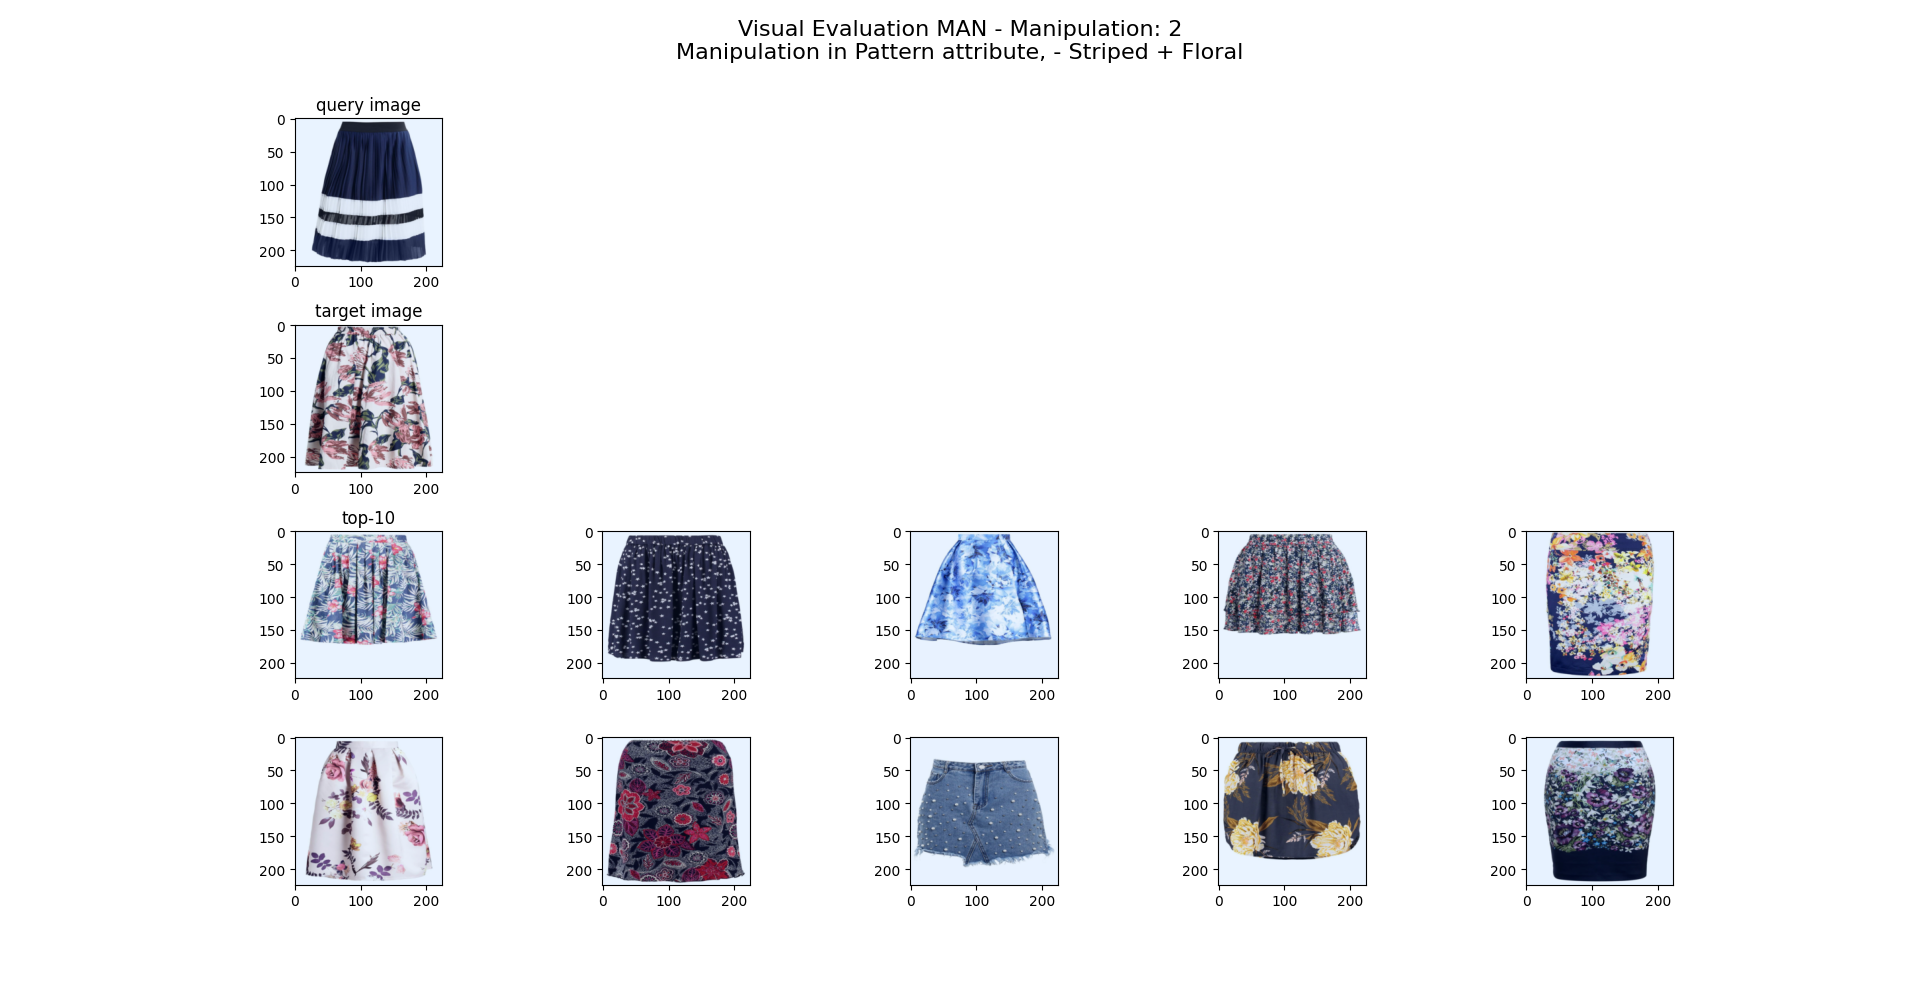
\includegraphics[scale=0.28]{"Immagini/3.2.png"}
 			\end{center}
\end{figure}
\item[] <3|only@3> 
\hspace{-20px}
\begin{figure}[!h]
 			\begin{center}
 			\hspace{-80px}
 			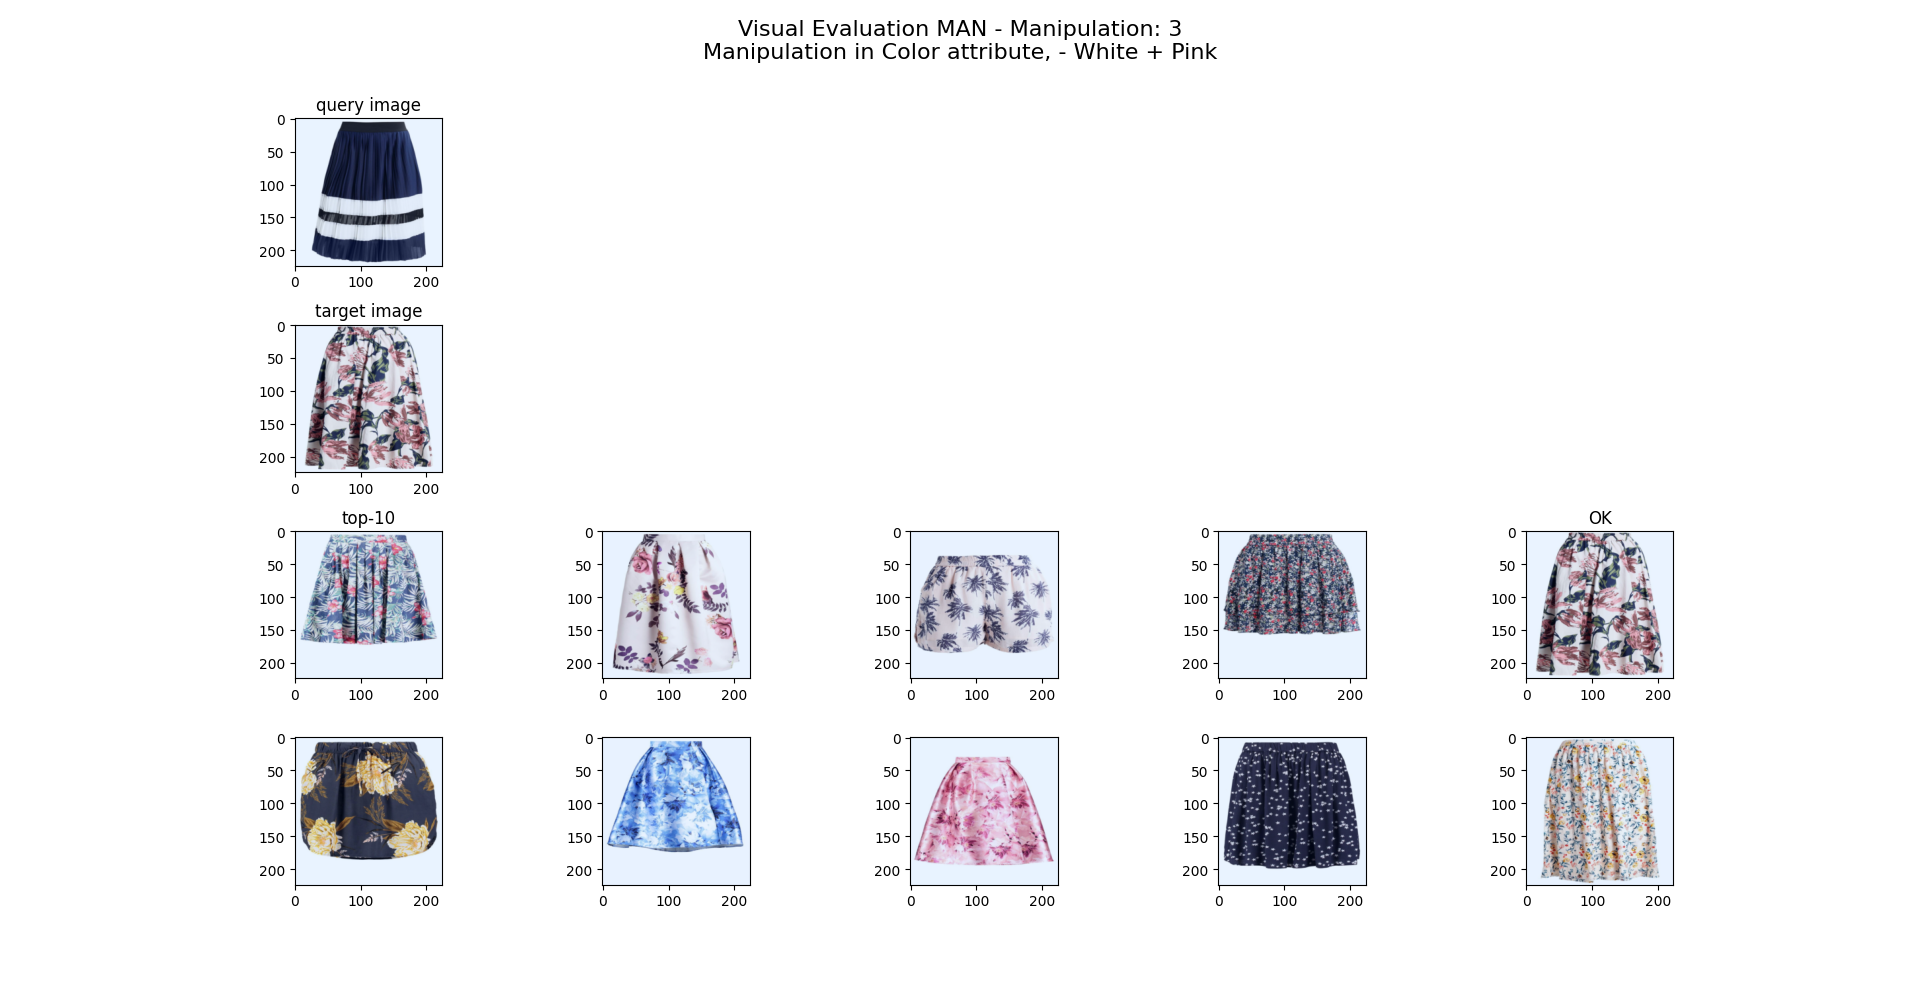
\includegraphics[scale=0.28]{"Immagini/3.3.png"}
 			\end{center}
\end{figure}
\item[] <4|only@4> 
\hspace{-20px}
\begin{figure}[!h]
 			\begin{center}
 			\hspace{-80px}
 			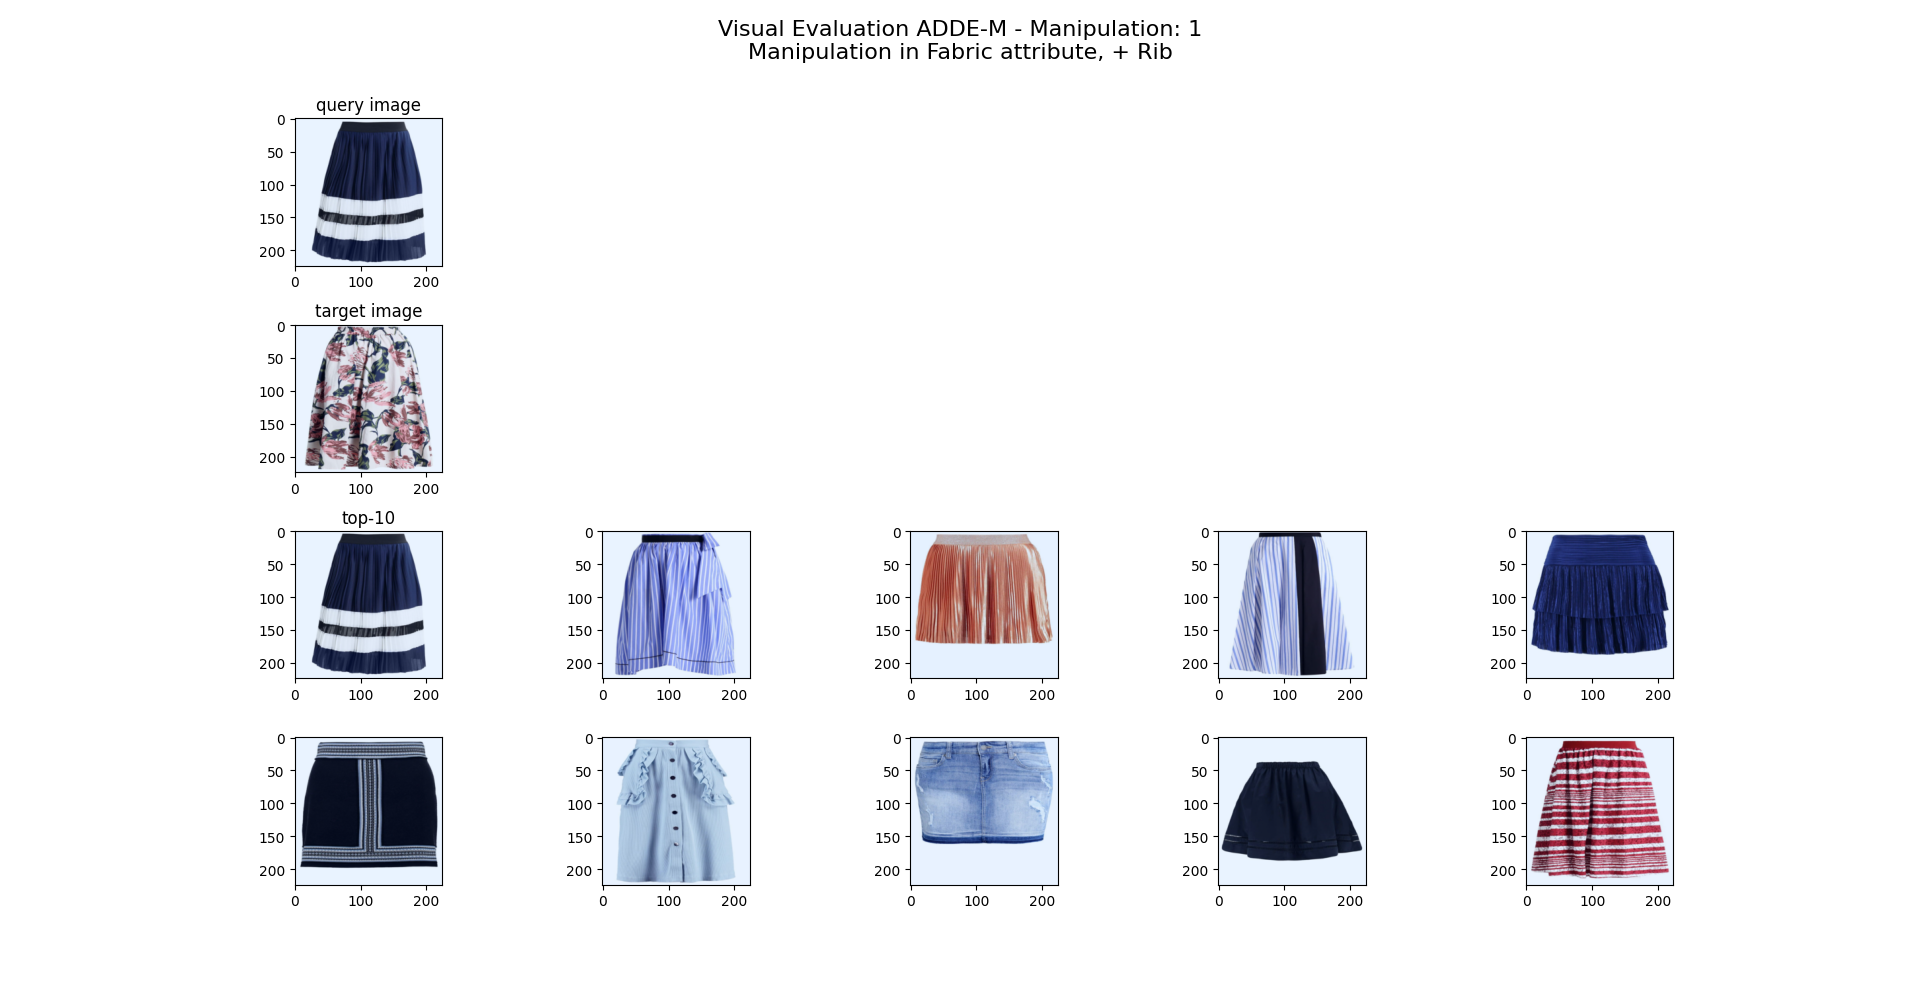
\includegraphics[scale=0.28]{"Immagini/3.4.png"}
 			\end{center}
\end{figure}
\item[] <5|only@5>
\hspace{-20px} 
\begin{figure}[!h]
 			\begin{center}
 			\hspace{-80px}
 			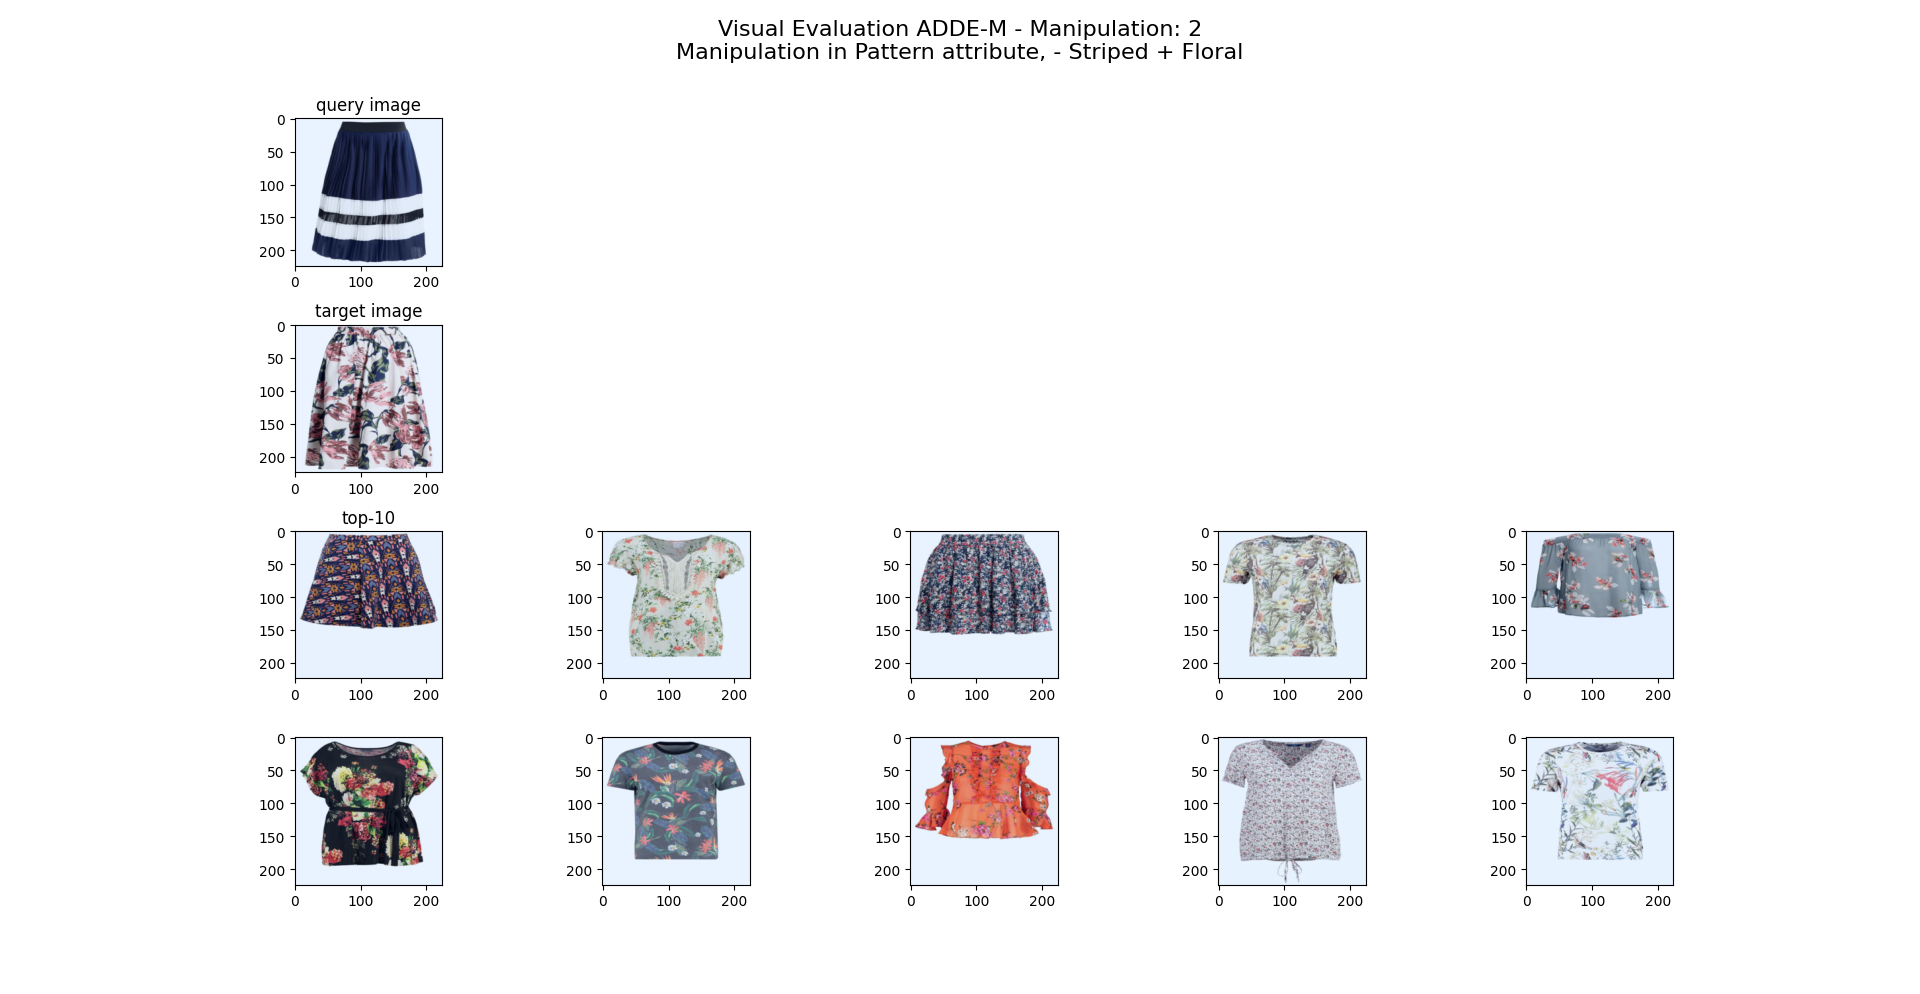
\includegraphics[scale=0.28]{"Immagini/3.5.png"}
 			\end{center}
\end{figure}
\item[] <6|only@6> 
\hspace{-20px}
\begin{figure}[!h]
 			\begin{center}
 			\hspace{-80px}
 			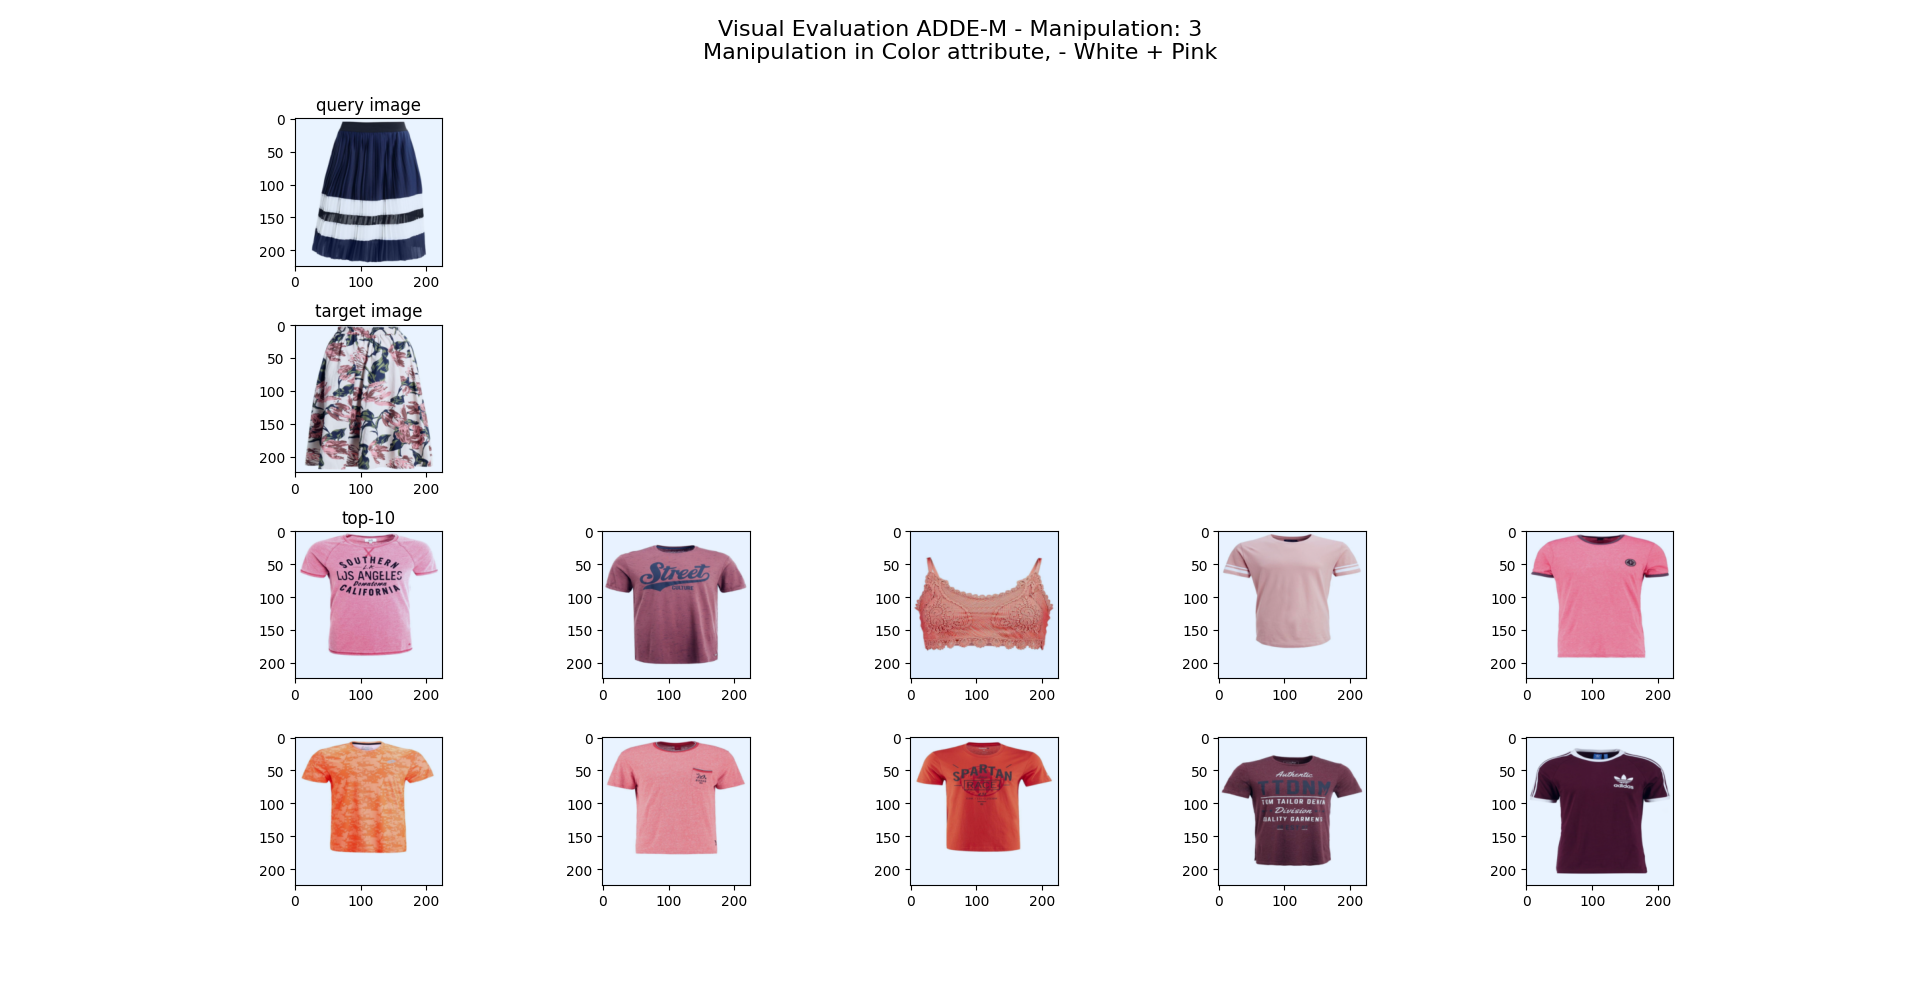
\includegraphics[scale=0.28]{"Immagini/3.6.png"}
 			\end{center}
\end{figure}
\end{itemize}
\end{frame}

\begin{frame}
\frametitle{Risultati}
\begin{itemize} 
\item Confronto visuale MANN e ADDE-M con $4$ manipolazioni
\item[] <1|only@1> 
\hspace{-20px}
\begin{figure}[!h]
 			\begin{center}
 			\hspace{-80px}
 			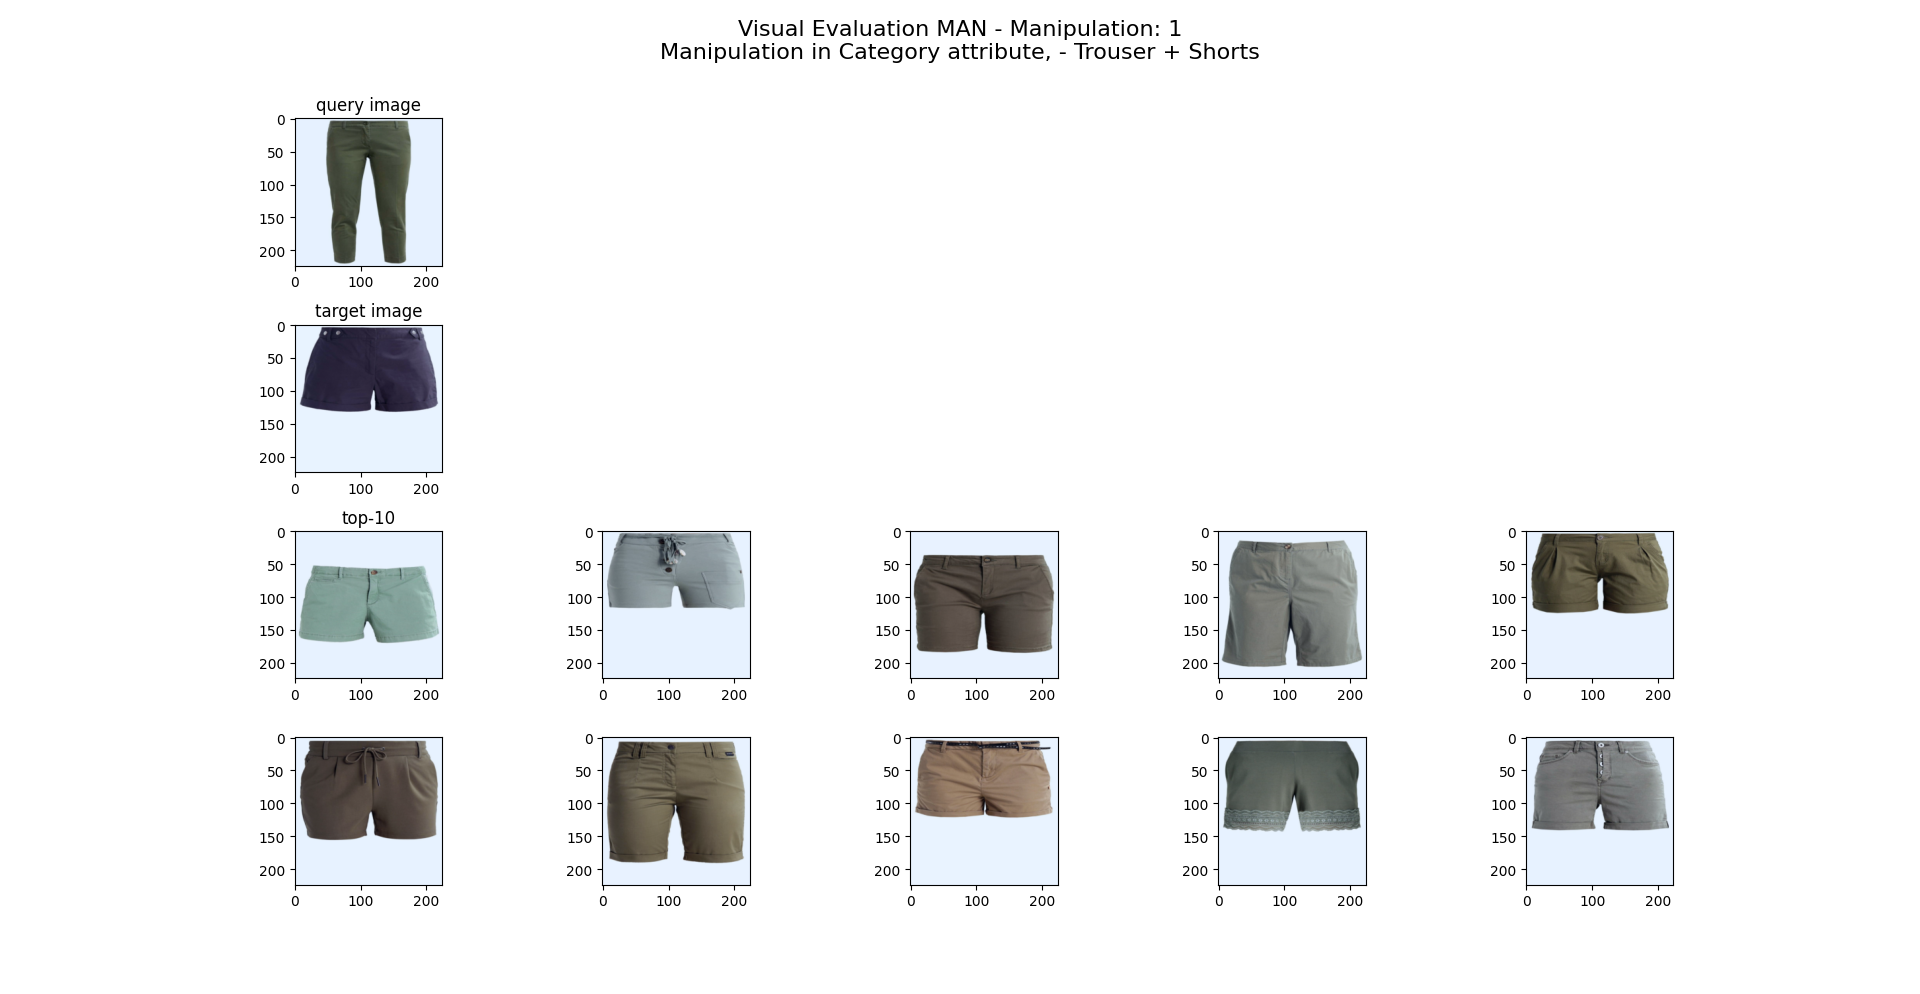
\includegraphics[scale=0.28]{"Immagini/4.1.png"}
 			\end{center}
\end{figure}
\item[] <2|only@2>
\hspace{-20px}
\begin{figure}[!h]
 			\begin{center}
 			\hspace{-80px}
 			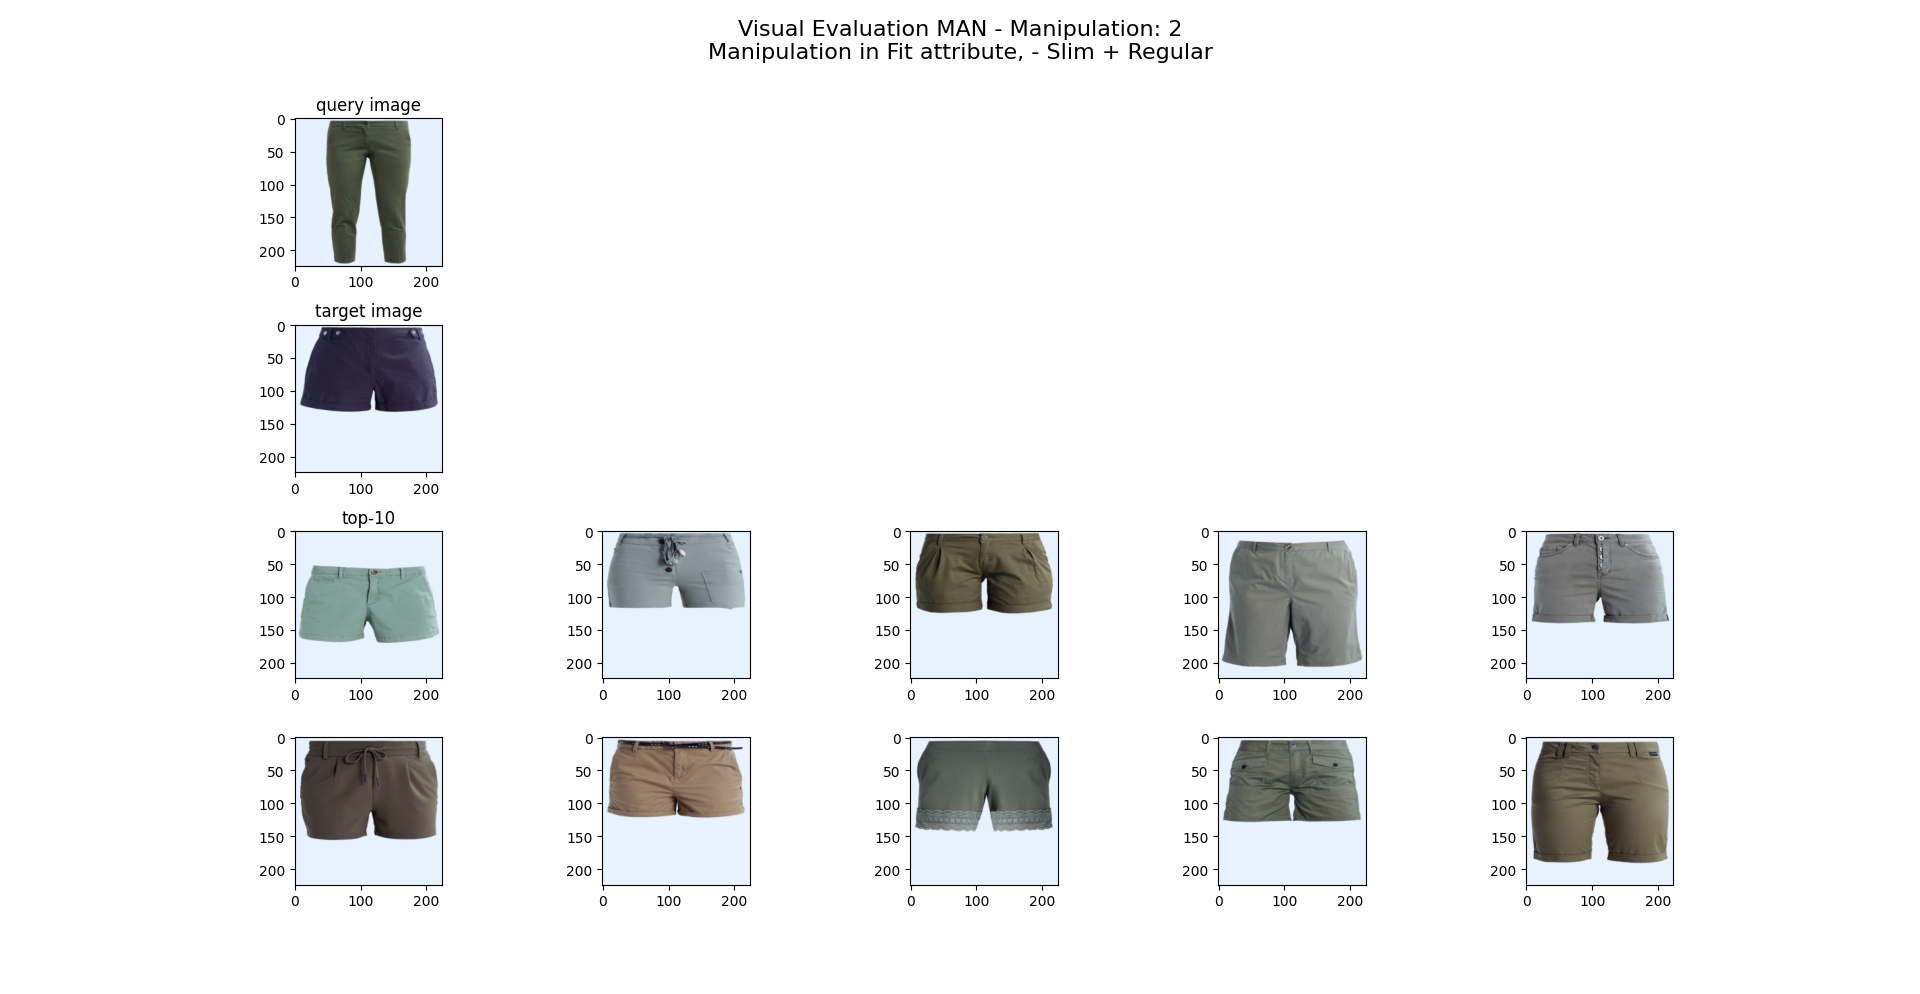
\includegraphics[scale=0.28]{"Immagini/4.2.png"}
 			\end{center}
\end{figure}
\item[] <3|only@3> 
\hspace{-20px}
\begin{figure}[!h]
 			\begin{center}
 			\hspace{-80px}
 			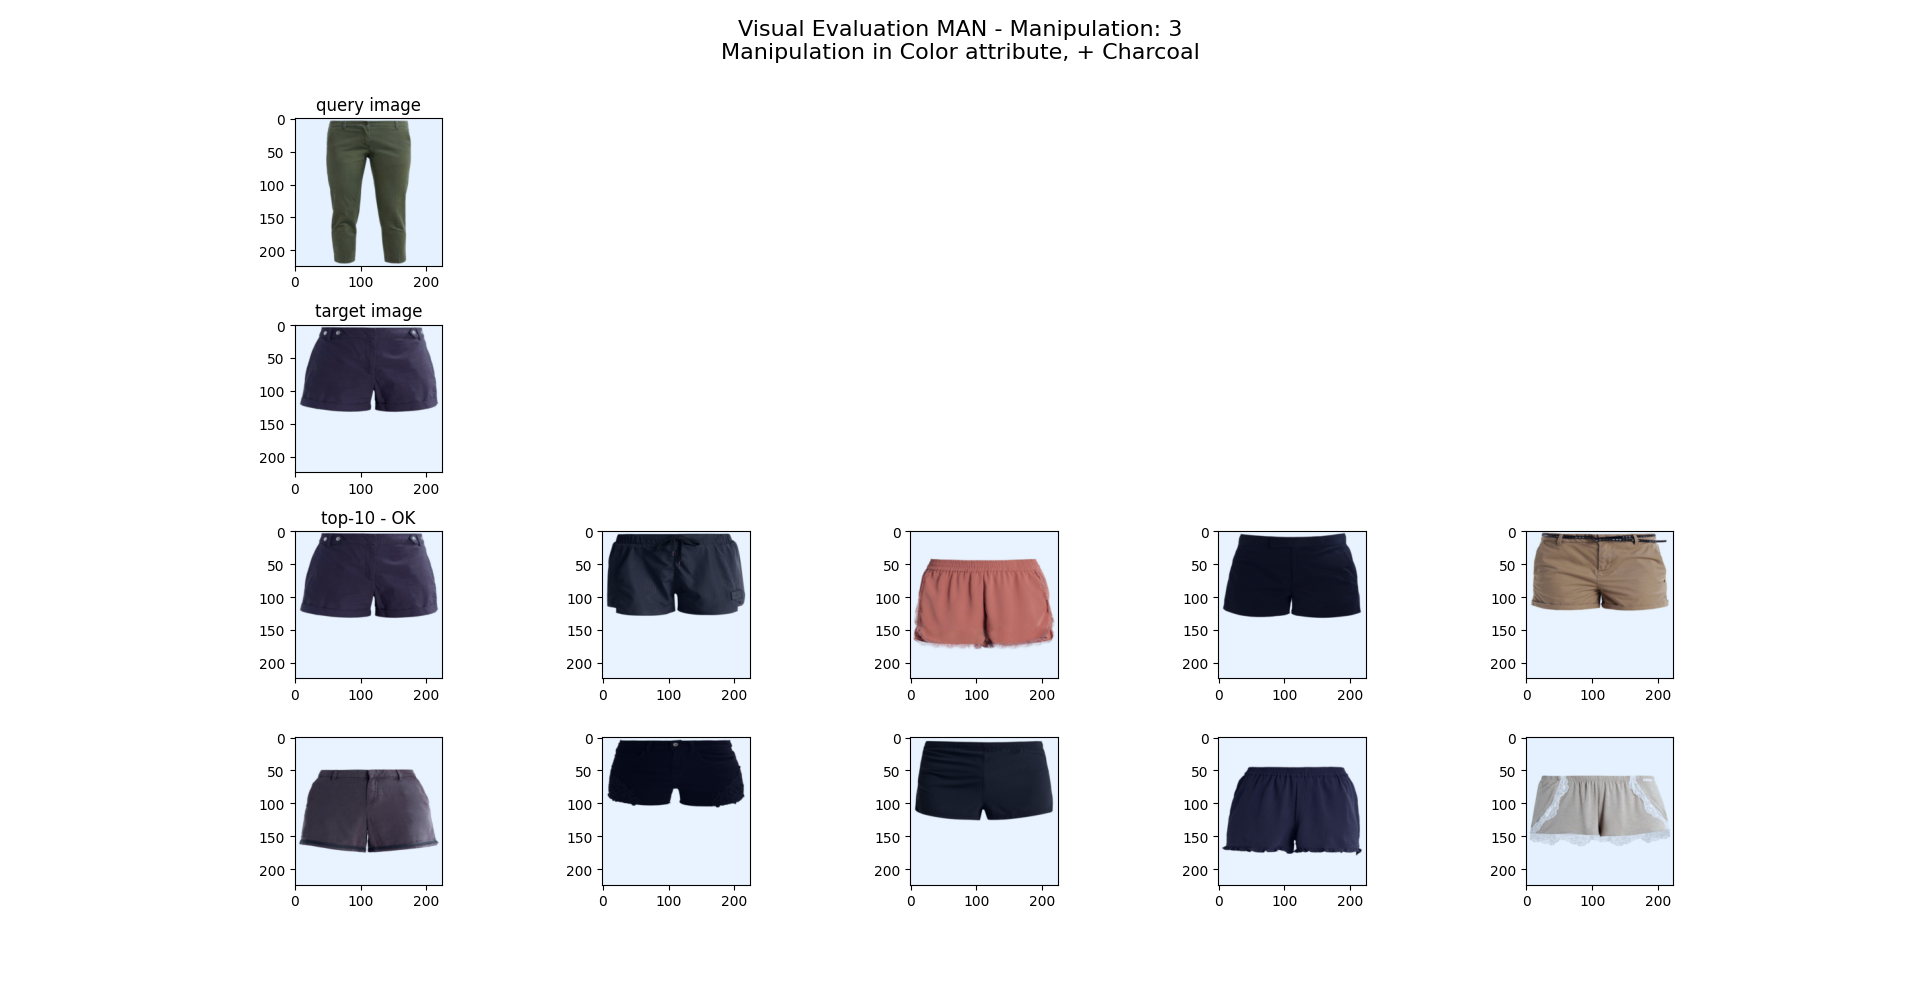
\includegraphics[scale=0.28]{"Immagini/4.3.png"}
 			\end{center}
\end{figure}
\item[] <4|only@4> 
\hspace{-20px}
\begin{figure}[!h]
 			\begin{center}
 			\hspace{-80px}
 			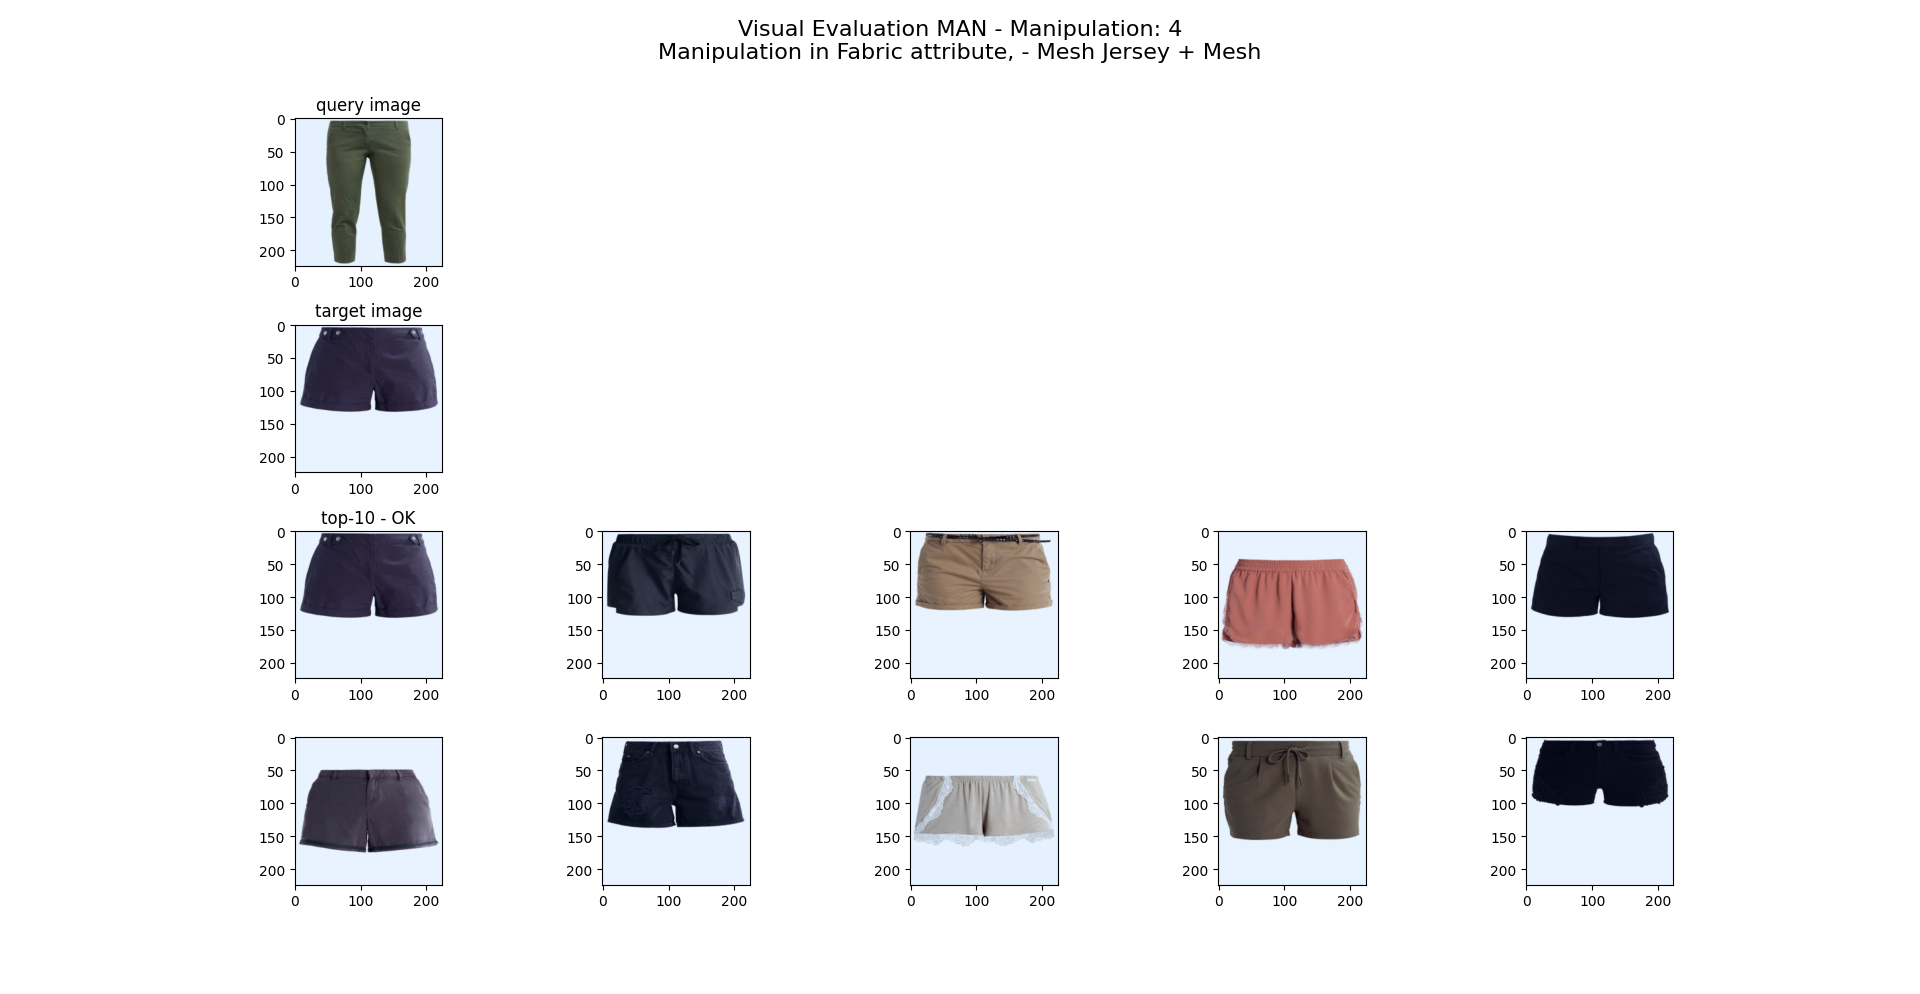
\includegraphics[scale=0.28]{"Immagini/4.4.png"}
 			\end{center}
\end{figure}
\item[] <5|only@5> 
\hspace{-20px}
\begin{figure}[!h]
 			\begin{center}
 			\hspace{-80px}
 			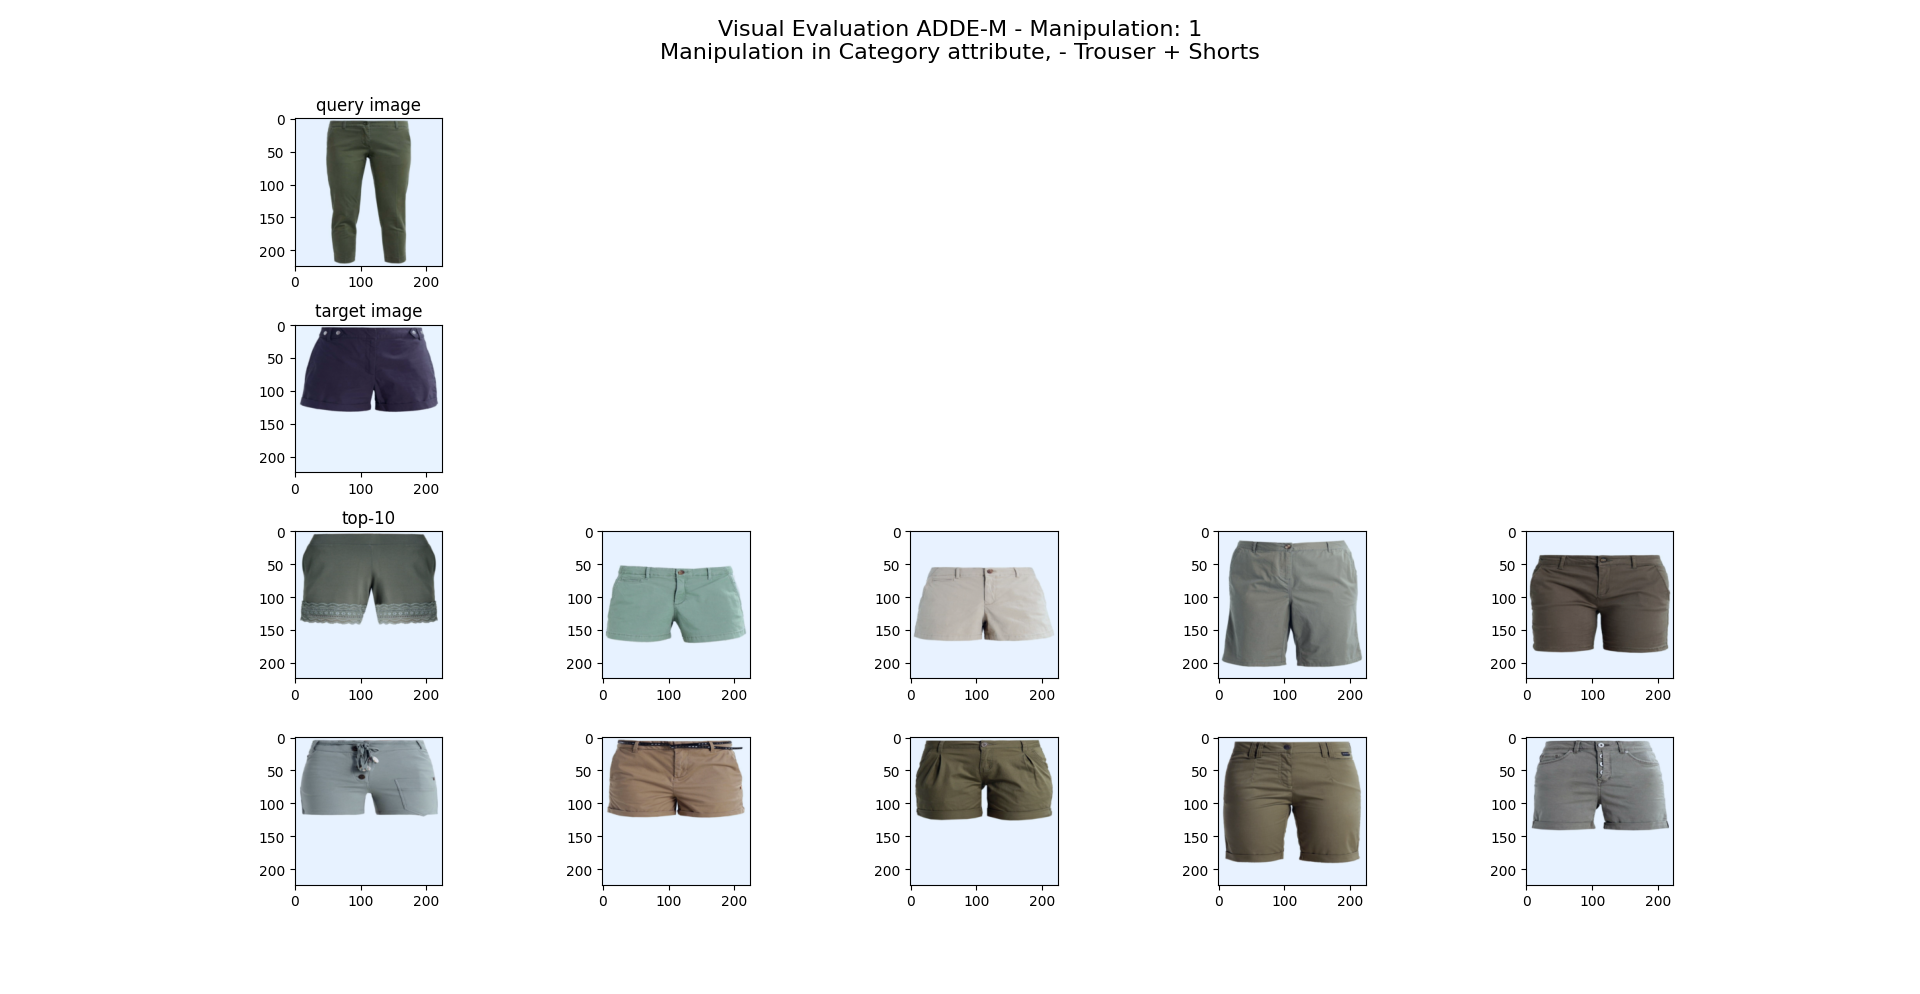
\includegraphics[scale=0.28]{"Immagini/4.5.png"}
 			\end{center}
\end{figure}
\item[] <6|only@6> 
\hspace{-20px}
\begin{figure}[!h]
 			\begin{center}
 			\hspace{-80px}
 			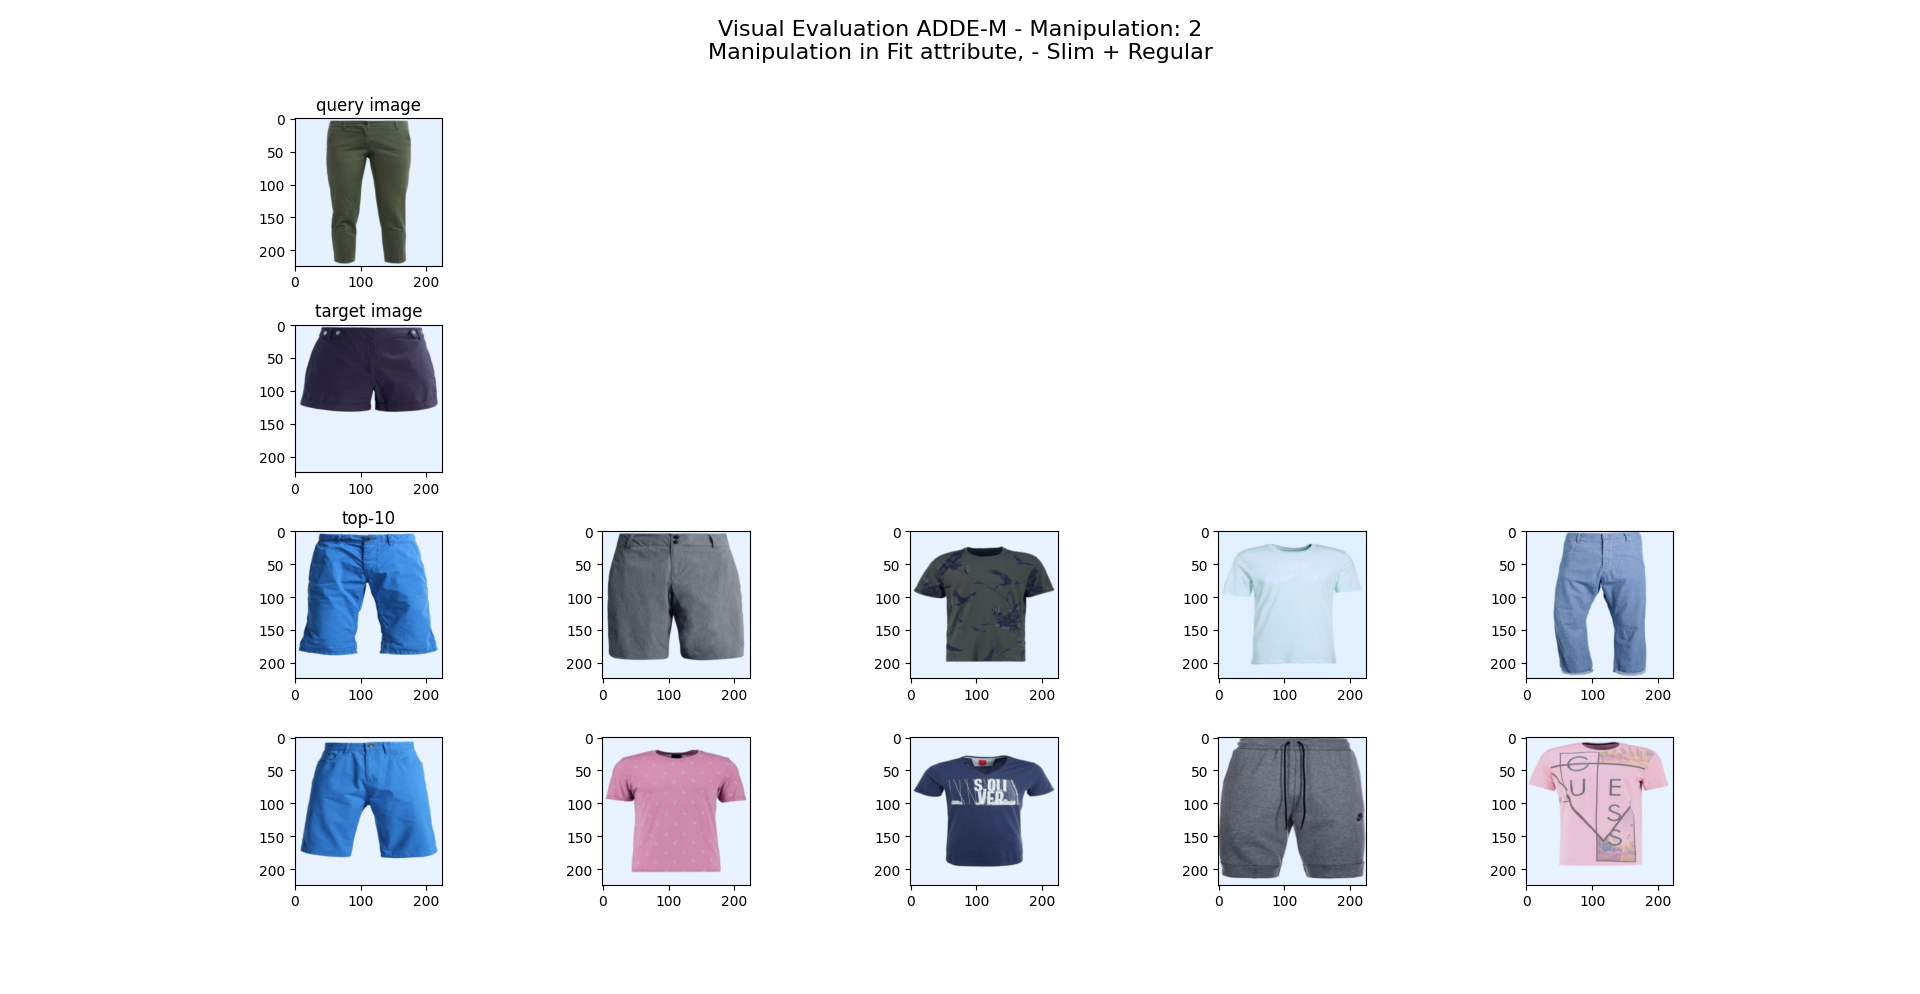
\includegraphics[scale=0.28]{"Immagini/4.6.png"}
 			\end{center}
\end{figure}
\item[] <7|only@7> 
\hspace{-20px}
\begin{figure}[!h]
 			\begin{center}
 			\hspace{-80px}
 			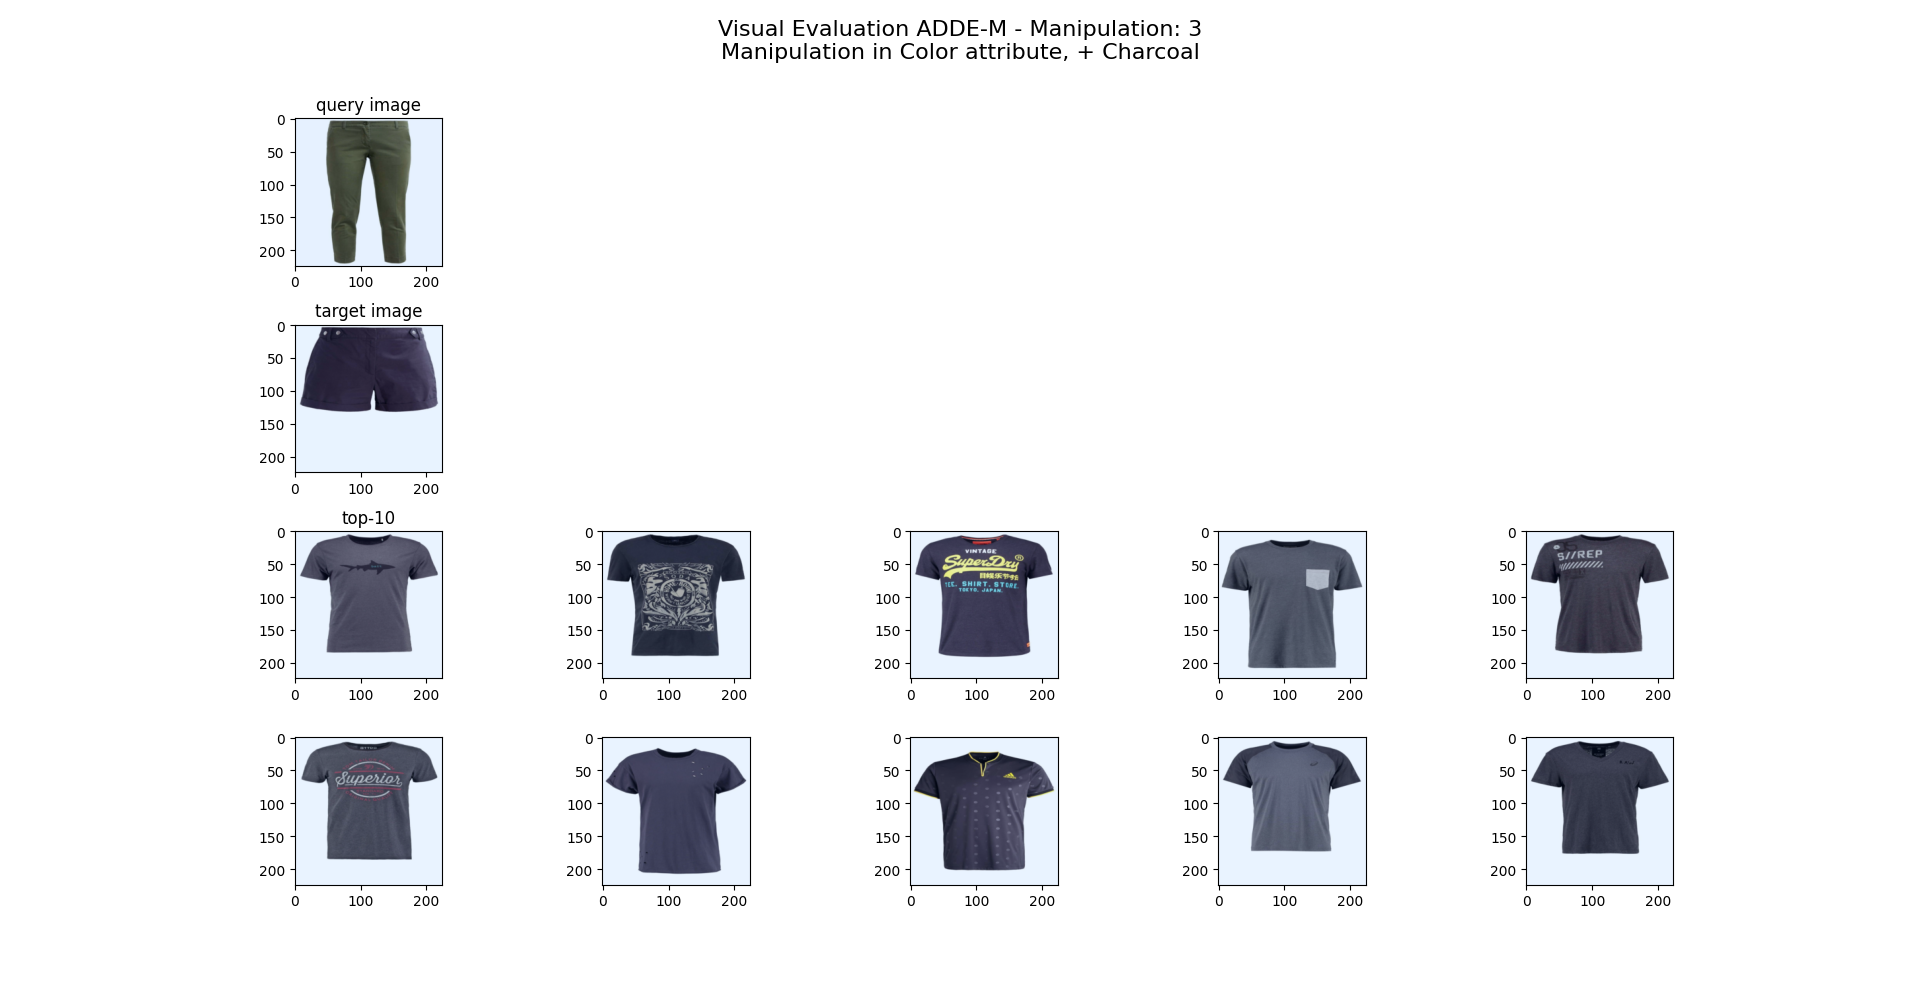
\includegraphics[scale=0.28]{"Immagini/4.7.png"}
 			\end{center}
\end{figure}
\item[] <8|only@8>
\hspace{-20px} 
\begin{figure}[!h]
 			\begin{center}
 			\hspace{-80px}
 			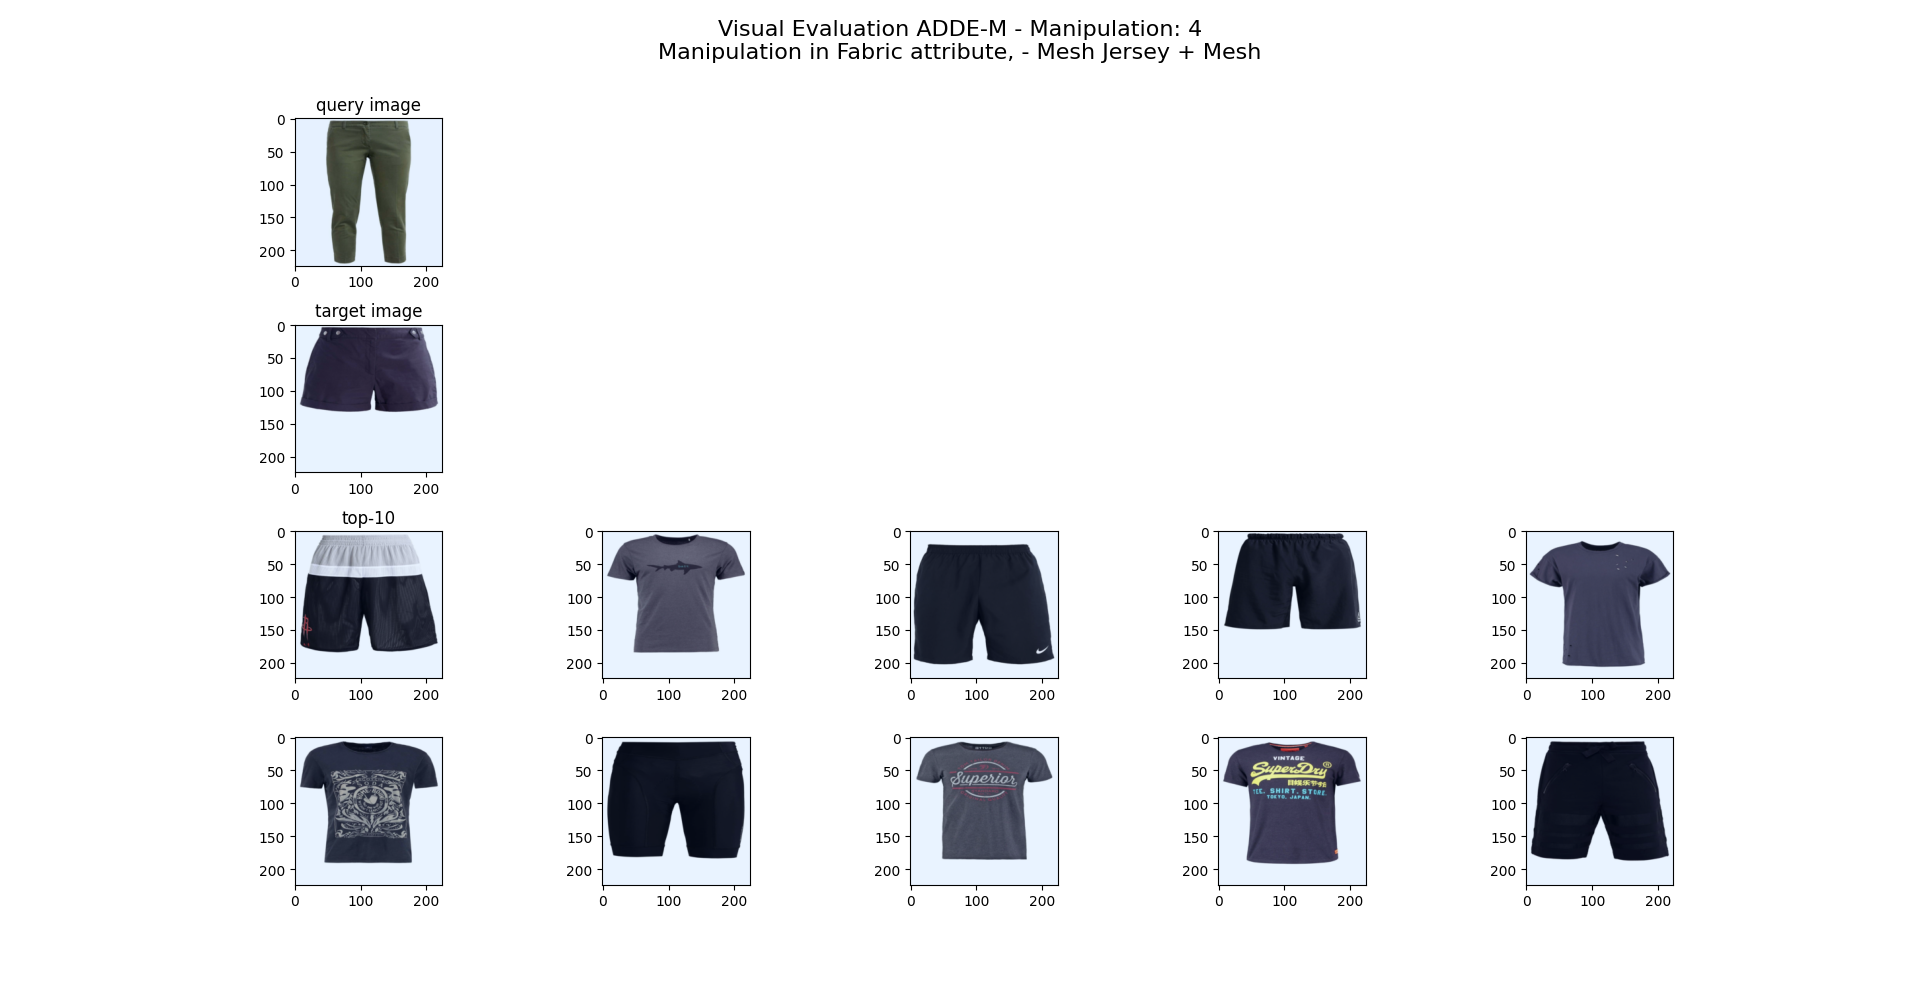
\includegraphics[scale=0.28]{"Immagini/4.8.png"}
 			\end{center}
\end{figure}
\end{itemize}
\end{frame}

\begin{frame}
\frametitle{Conclusioni}
\begin{itemize}
\item Memory Augmented Neural Network per task di manipolazione su immagini di vestiti
\item Semplicit\'a del modello $\Rightarrow$ Performance inferiore su una singola manipolazione
\item Memoria esterna indipendente e indirizzabile $\Rightarrow$ Performance maggiore su pi\'u manipolazioni in sequenza
\end{itemize}
\begin{figure}[!h]
 			\begin{center}
 			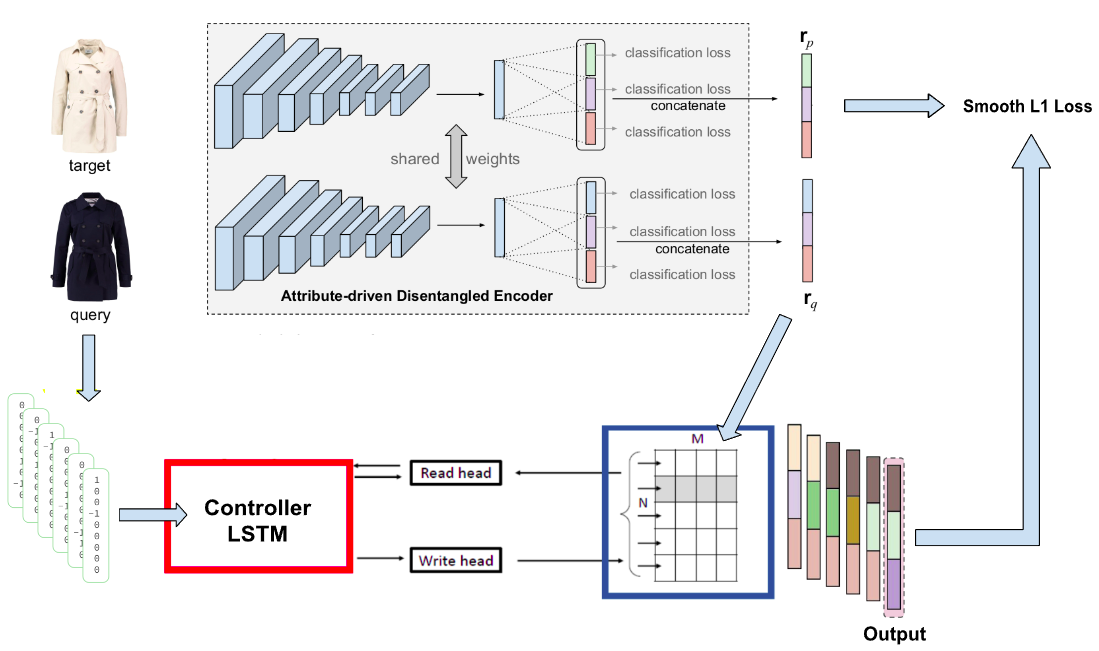
\includegraphics[scale=0.20]{"Immagini/All2.png"}
 			\end{center}
\end{figure}
\end{frame}

\end{document}